\section{Experimentation}\label{sec:experiments}
% Backprop in ReLU can only propagate through the positive half-space
% Units and points lying on the negative side of the hyperplanes are thus bound to fail.
Using back-propagation in \ReLU networks can only propagate through the positive half-space
\begin{enumerate}
    \item Force units to separate at least two points.
    \item Force points to have at least one positive and negative pre-activation. . 
\end{enumerate}

Hypothesis at hand:\\\\
In the case of \ReLU based DNN, we claim that these issues have a geometric undertow, that corrupts back-propagation as a training strategy. To be more precise, we contend that gradient issues (vanishing and exploding) alongside with death problems (unit and point) are intertwined with the position of the hyper-planes defined by the preactivation of \ReLU units, that hinders error minimization.
\begin{enumerate}
    \item correctly positioning units to make them separation units following the definitions on subsection \ref{subsec:ReLUSeparability}.
    \item ensuring that each point in the data-set is separated contrarily by at least two units. That is, it lies on the affine component of one, and on the zero-set of another. 
\end{enumerate}
\subsection{Performance assessment}\label{subsec:benchmarking}
In terms of overall performance, we chose to benchmark the separating constraints against one another, and to the very popular \emph{batch normalization} as presented in \cite{batchnorm} using the implementation from \texttt{Keras}. 
\\\\
The reader can find a summary  of overall results in Table \ref{tab:moons}. The highest performance was obtained by the \SepLayer with an accuracy of $100\%$ both in validation and training, and attaining a loss value of $0$ in training. While the separation constraints display superior accuracy in comparison to classical \ReLU and batchnorm (first two rows of Table \ref{tab:moons}), it is important to notice that the accuracy drop between training and validation is also significantly lower percentage-wise. While classical \ReLU and \ReLUBN experience a $20+\%$ accuracy drop between training and validation, the \SepConstraint family experiences drops from less than $14\%$, with \SepUnitPoint experiencing only a $5,59\%$ accuracy drop.  
\\\\
However, Loss value variation (recorded at maximal accuracy performance) is significantly higher using for the \SepConstraint family ($72+\%$ for \SepUnit and \SepPoint and $100\%$ for \SepLayer), while for \ReLU and \ReLUBN loss variation remains below $5\%$. These measurements were taken for the \moons dataset using a fixed thin network of depth $D=50$ and a width $W=4$. 
\begin{table}[h!]
\begin{center}
\begin{tabular}{l|rr|rr}
\toprule
{}  & \multicolumn{2}{c}{Accuracy} & \multicolumn{2}{c}{Loss} \\
{}  & Train   & Val.  & Train  & Val.  \\
\midrule
\ReLU            &  0.5176 &      0.4 &  0.6925 &  0.6938 \\
\ReLUBN     &  0.8117 &      0.6 &  0.6331 &  0.6636 \\
\SepLayer &  1.0000 &      1.0 &  0.0000 &  0.0211 \\
\SepPoint    &  0.9294 &  0.8000 &  0.1765 &  0.6476 \\
\SepUnit    &  0.9058 &  0.8000 &  0.4161 &  1.5228 \\
\SepUnitPoint   &  0.9882 &  0.9333 &  0.6988 &  1.0810 \\
\bottomrule
\end{tabular}
\end{center}
\caption{Maximal performance experiment using the \moons dataset. From left to right, accuracy and loss (for \emph{train} and \emph{validation} sets) for \ReLU, \ReLUBN, and  \SepConstraint in all its variants.}
  \label{tab:moons}
\end{table}

When varying depth and width we can see that the \SepConstraint Family works favorably in deeper thin networks. Notice how \ReLU, Figure \ref{fig:moons_grid_relu}, fails with networks deeper than 30 layers. In other hand, \ReLUBN, Figure \ref{fig:moons_grid_relubn}, manages to work until 70 layers deep. \SepUnitPoint,  Figure \ref{fig:moons_grid_up}, works significantly better than both, up to 120 layers. Notice how all the methods suffer from depth-dependent accuracy degradation, but is compensated (partially) using width increase. This is consistent with \cite{simpnet} and \cite{densenet}. 
\\\\
\SepUnitPoint however is able to delay the apparition of the issue. Specially when using \emph{skinny} DNN ($W$ in between $2$ to $5$) where \ReLUBN fails. We observe that \SepUnit, Figure \ref{fig:moons_grid_u}, allows for deeper networks yet accuracy drops inversely to width, a phenomenon we blaim on the inability of the \SepUnit constraint to address the \emph{dead points}. 
\\\\
In addition, \SepPoint, (Figure \ref{fig:moons_grid_p}), seems to perform well up to 50 layers, but it breaks down afterwards. Finally, \SepLayer (Figure \ref{fig:moons_grid_l}) seems to suffer most with larger widths (after 25), but can also mantain acceptable performance levels well into 70 layers with a medium width.
\begin{figure*}[h!]
  \centering
    \begin{subfigure}[b]{0.3\textwidth}
        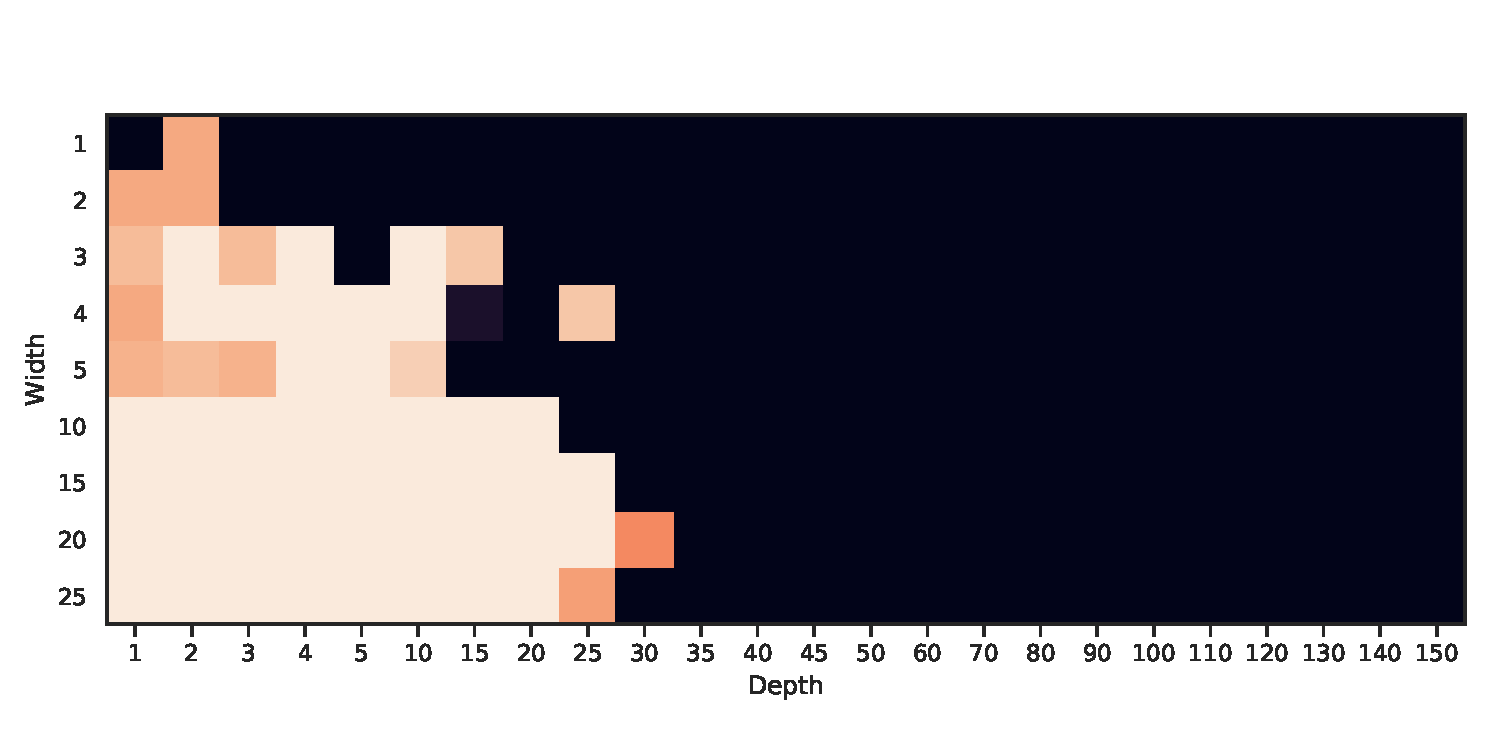
\includegraphics[width=\textwidth]{img/moons_grid/acc-relu.pdf}
        \caption{\ReLU}
        \label{fig:moons_grid_relu}
    \end{subfigure}
    ~ %add desired spacing between images, e. g. ~, \quad, \qquad, \hfill etc. 
      %(or a blank line to force the subfigure onto a new line)
    \centering
    \begin{subfigure}[b]{0.3\textwidth}
        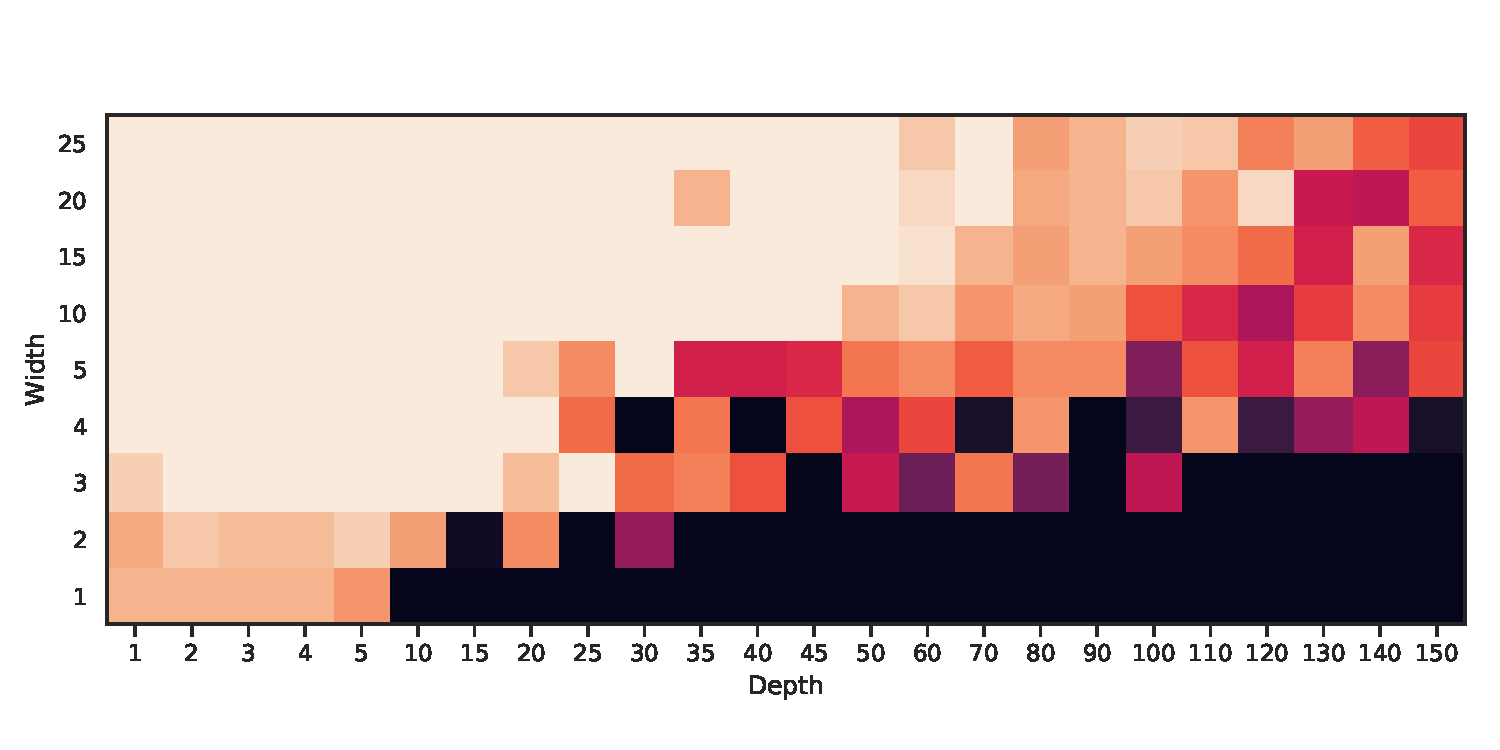
\includegraphics[width=\textwidth]{img/moons_grid/acc-relu-bn.pdf}
        \caption{\ReLUBN}
        \label{fig:moons_grid_relubn}
    \end{subfigure}
    ~ %add desired spacing between images, e. g. ~, \quad, \qquad, \hfill etc. 
      %(or a blank line to force the subfigure onto a new line)
    \centering
    \begin{subfigure}[b]{0.3\textwidth}
        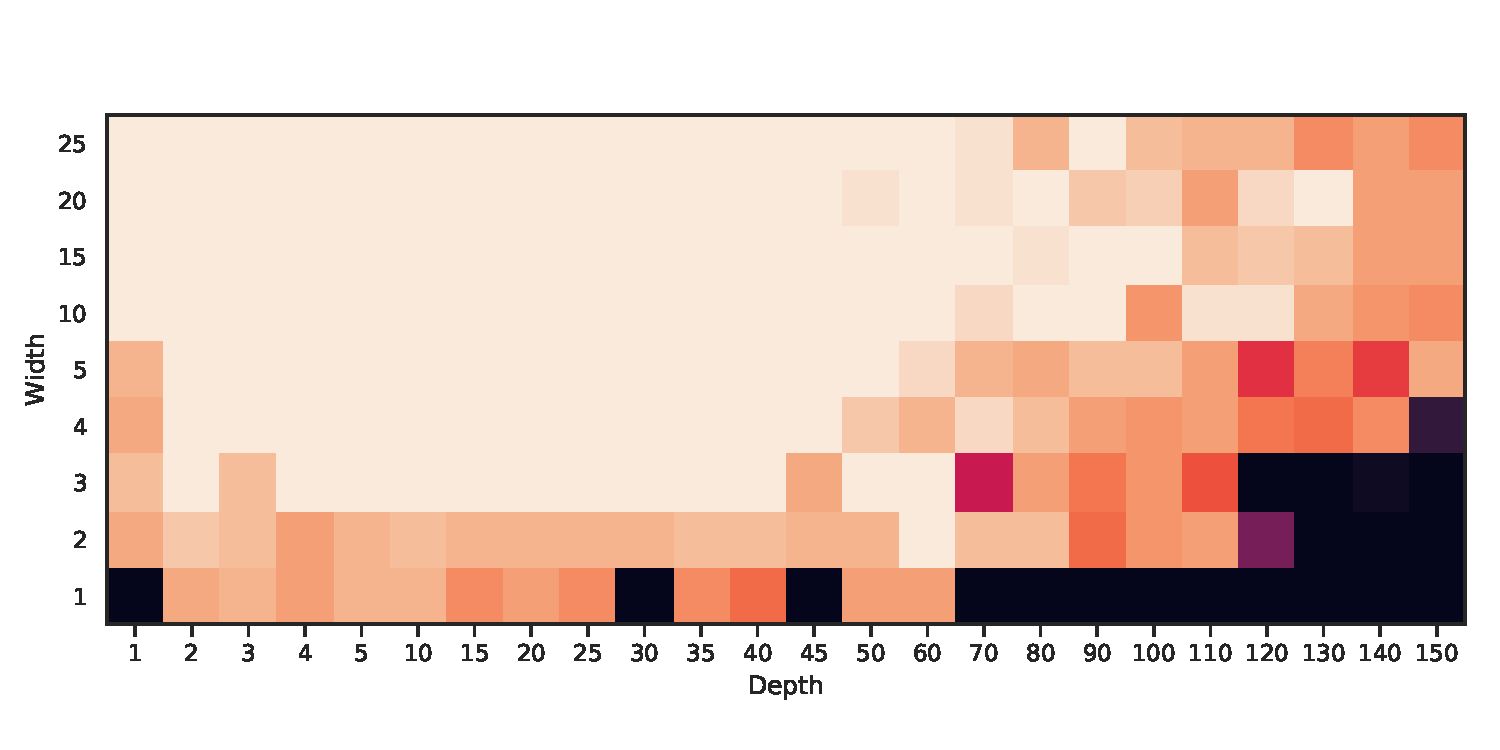
\includegraphics[width=\textwidth]{img/moons_grid/acc-sep-up-0-0001.pdf}
        \caption{\SepUnitPoint}
        \label{fig:moons_grid_up}
    \end{subfigure}
    ~ %add desired spacing between images, e. g. ~, \quad, \qquad, \hfill etc. 
      %(or a blank line to force the subfigure onto a new line)
    \\
    \begin{subfigure}[b]{0.3\textwidth}
        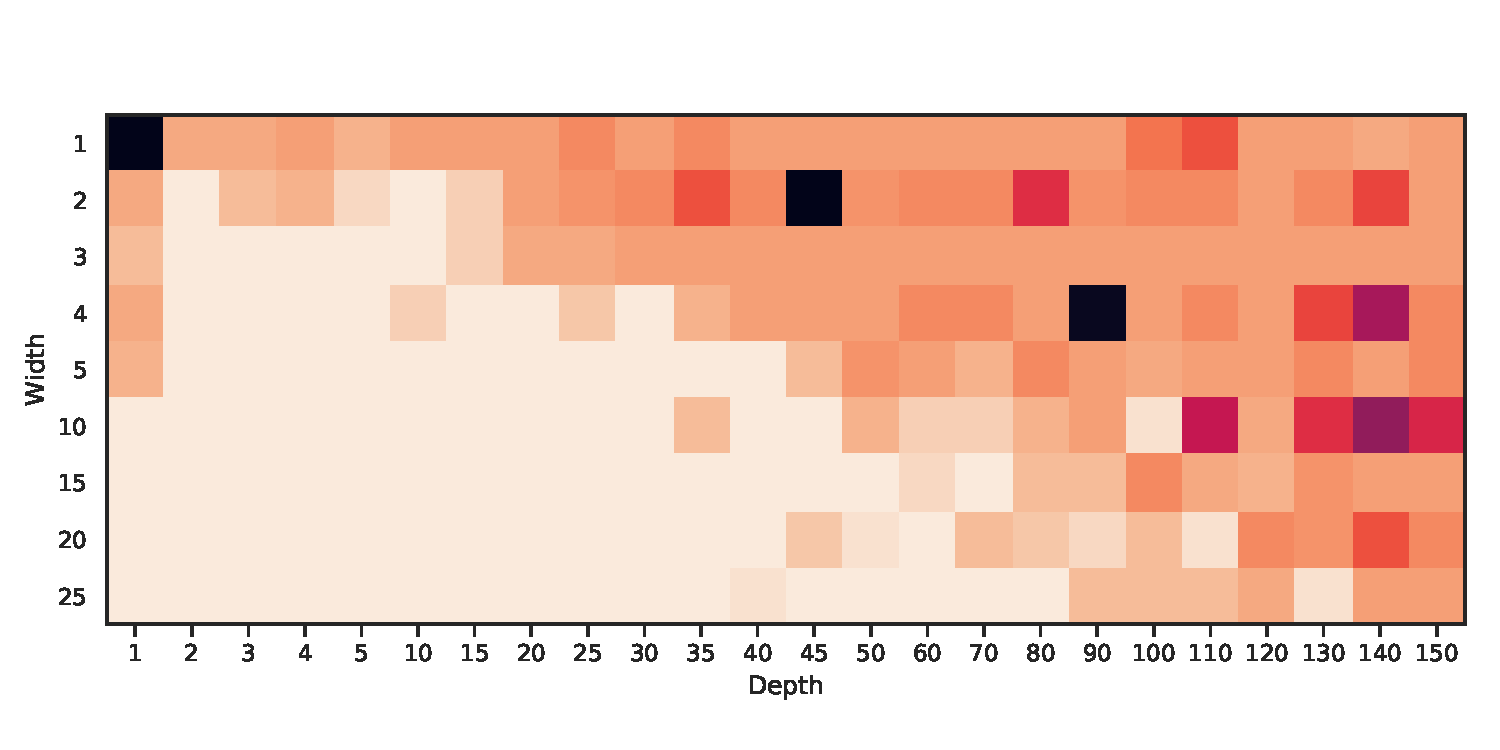
\includegraphics[width=\textwidth]{img/moons_grid/acc-sep-u-0-0001.pdf}
        \caption{\SepUnit}
        \label{fig:moons_grid_u}
    \end{subfigure}
    ~ %add desired spacing between images, e. g. ~, \quad, \qquad, \hfill etc. 
      %(or a blank line to force the subfigure onto a new line)
    \centering
    \begin{subfigure}[b]{0.3\textwidth}
        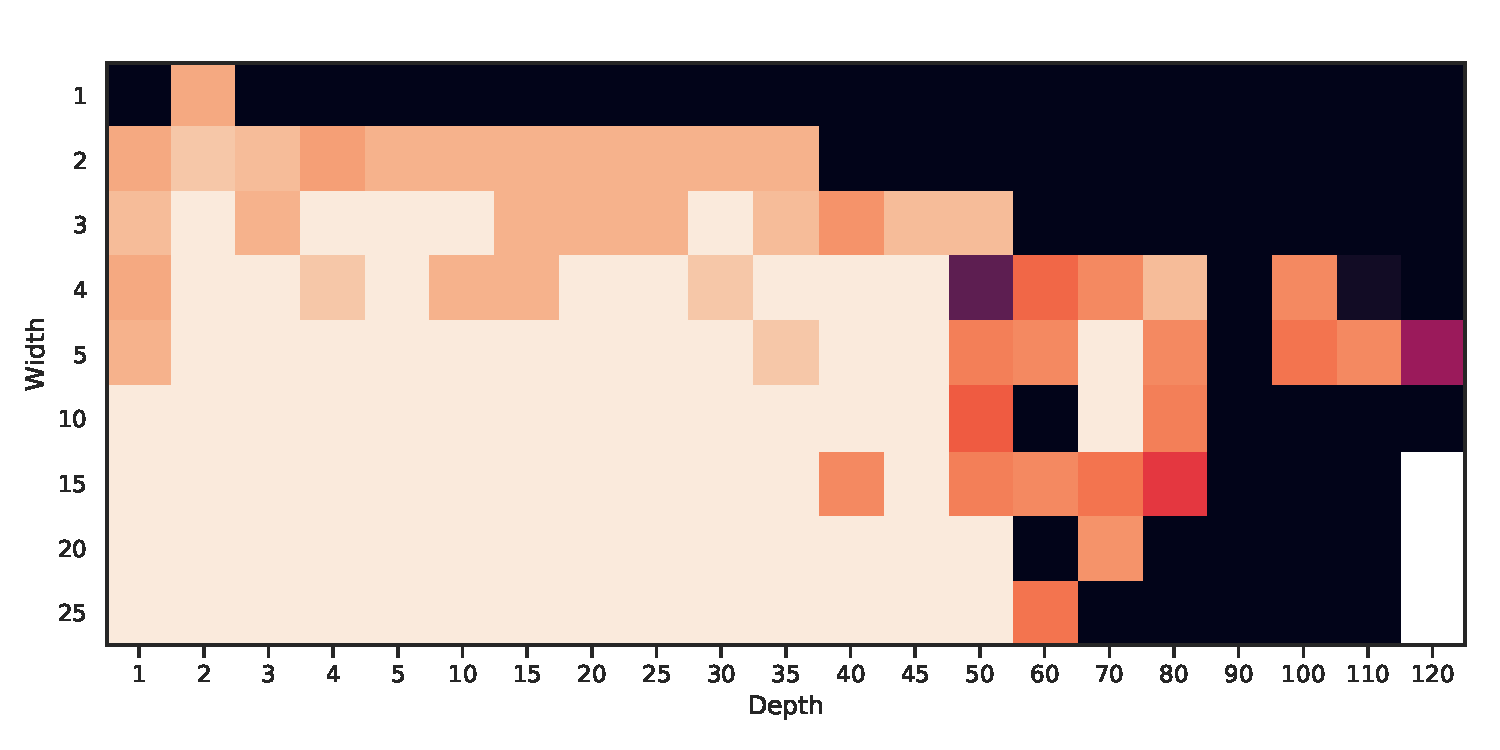
\includegraphics[width=\textwidth]{img/moons_grid/acc-sep-p-0-0001.pdf}
        \caption{\SepPoint}
        \label{fig:moons_grid_p}
    \end{subfigure}
    ~ %add desired spacing between images, e. g. ~, \quad, \qquad, \hfill etc. 
      %(or a blank line to force the subfigure onto a new line)
    \centering
    \begin{subfigure}[b]{0.3\textwidth}
        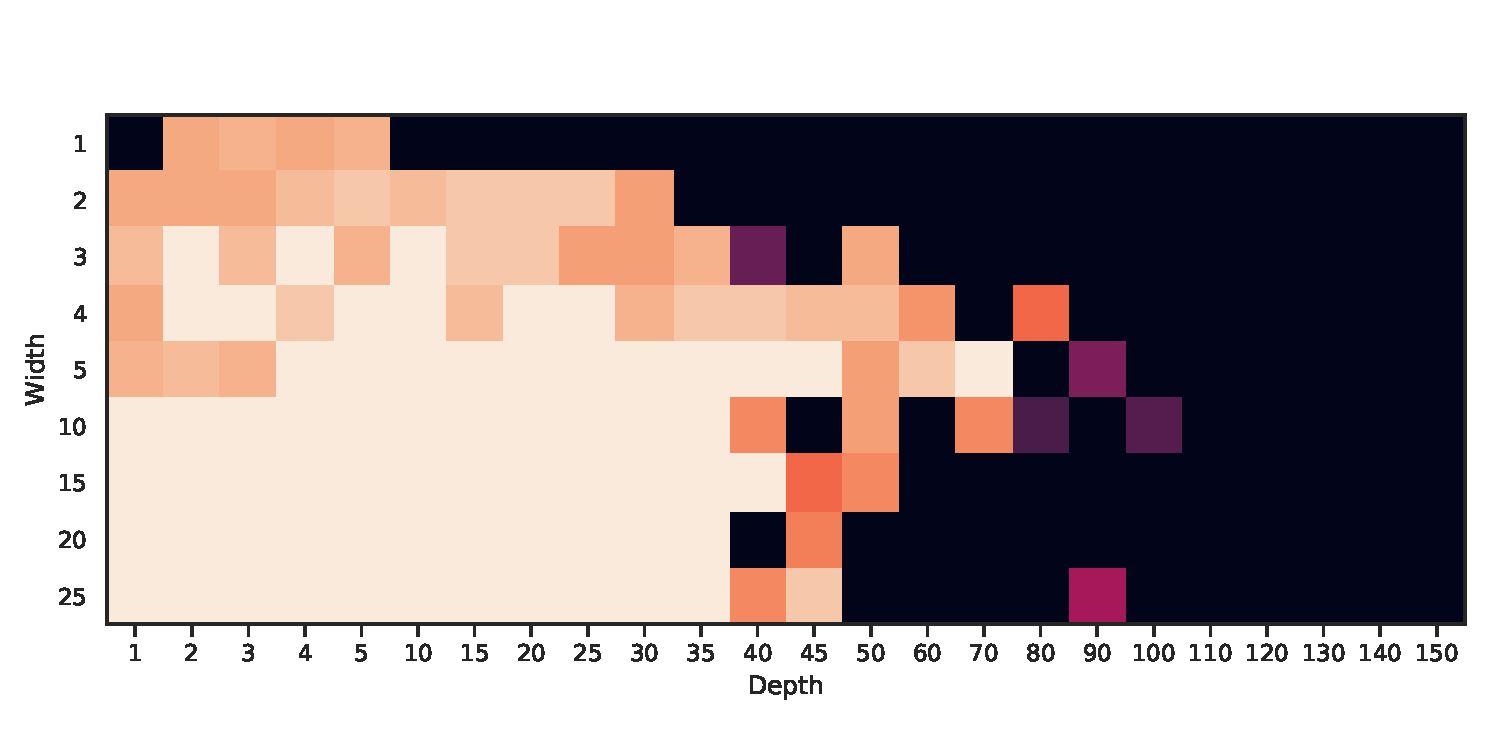
\includegraphics[width=\textwidth]{img/moons_grid/acc-sep-l-0-0001.pdf}
        \caption{\SepLayer}
        \label{fig:moons_grid_l}
    \end{subfigure}
    ~ %add desired spacing between images, e. g. ~, \quad, \qquad, \hfill etc. 
      %(or a blank line to force the subfigure onto a new line)
    
  \caption{Depth vs Width accuracy plot for a rectangular network of depth $W$ and depth $D$ varying both parameters: $2\leq W\leq 25$ and $2\leq D\leq 150$, over the \texttt{MOONS} dataset. This network were trained using an Adam scheme, and learning rate of $\gamma = 0.01$. The color map varies according to accuracy attained of each of the combinations of $W$ and $D$ (black is trivial accuracy and light cream is $1.0$)} 
  \label{fig:moons_grid} 
\end{figure*}
\subsection{On the geometry of the separation constraints}\label{subsec:geometryOfSeparation}

\begin{figure*}[h!]
  \centering
  \parbox{\textwidth}{
    \parbox{.195\textwidth}{%
      \subcaptionbox{Input layer\label{fig:moonsReLUInput}}{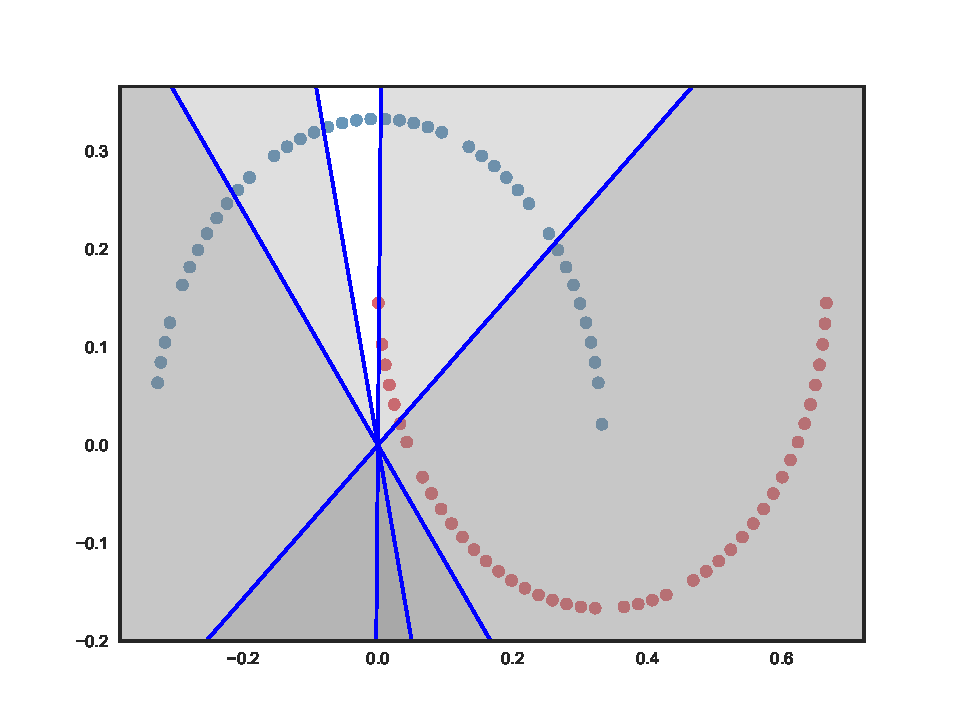
\includegraphics[width=\hsize]{img/toy/relu/conv2d_1-0.pdf}}
    }
    % \hskip1em
    \parbox{.195\textwidth}{%
      \subcaptionbox{4th layer\label{fig:moonsReLU41}}{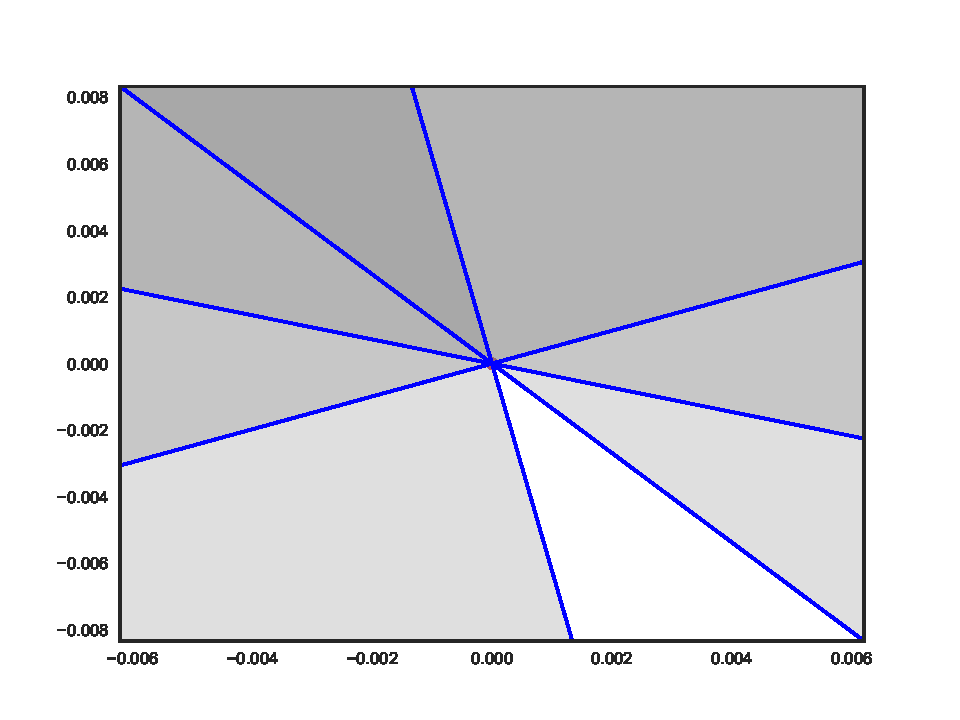
\includegraphics[width=\hsize]{img/toy/relu/conv2d_4-0.pdf}}
    %   \vskip1em
      \subcaptionbox{4th layer\label{fig:moonsReLU42}}{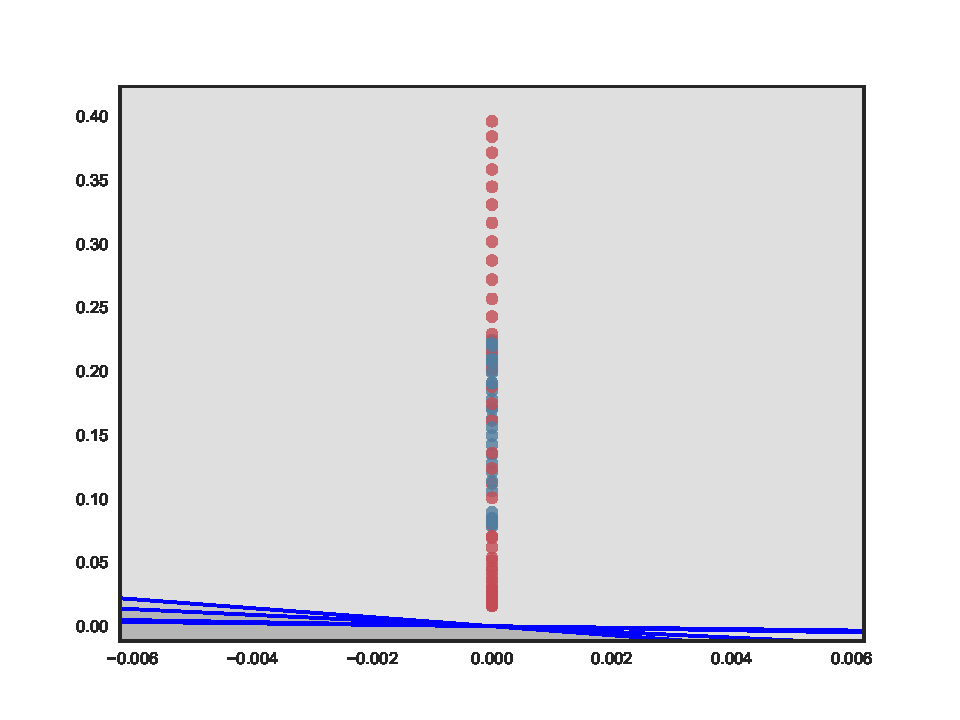
\includegraphics[width=\hsize]{img/toy/relu/conv2d_4-2.pdf}}
    }
    % \hskip1em
    \parbox{.195\textwidth}{%
      \subcaptionbox{25th layer\label{fig:moonsReLU251}}{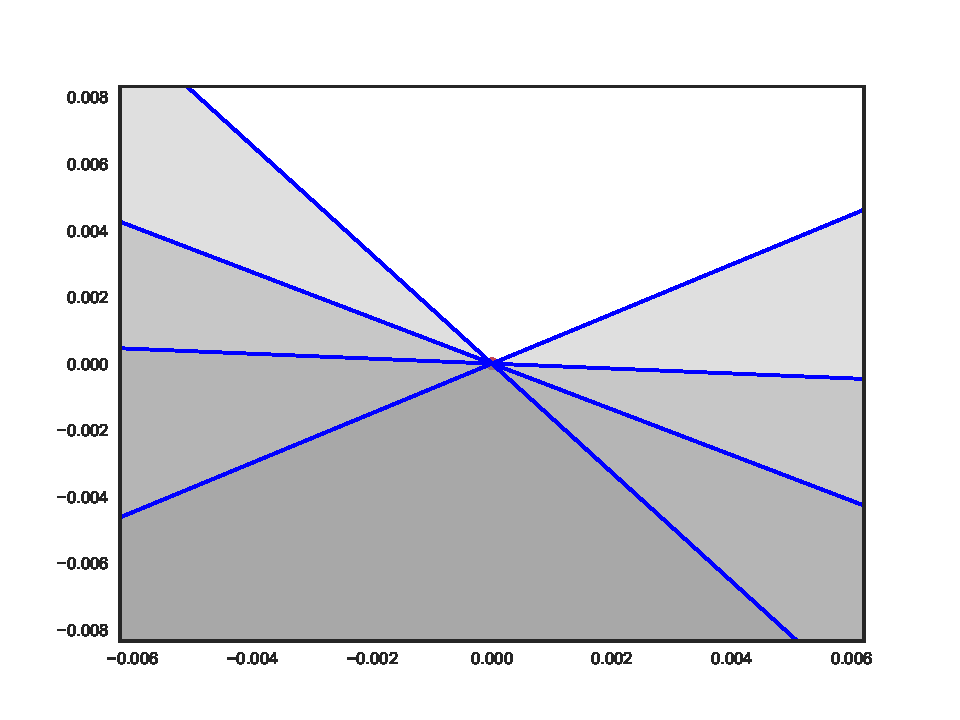
\includegraphics[width=\hsize]{img/toy/relu/conv2d_25-0.pdf}}
    %   \vskip1em
      \subcaptionbox{25th layer\label{fig:moonsReLU252}}{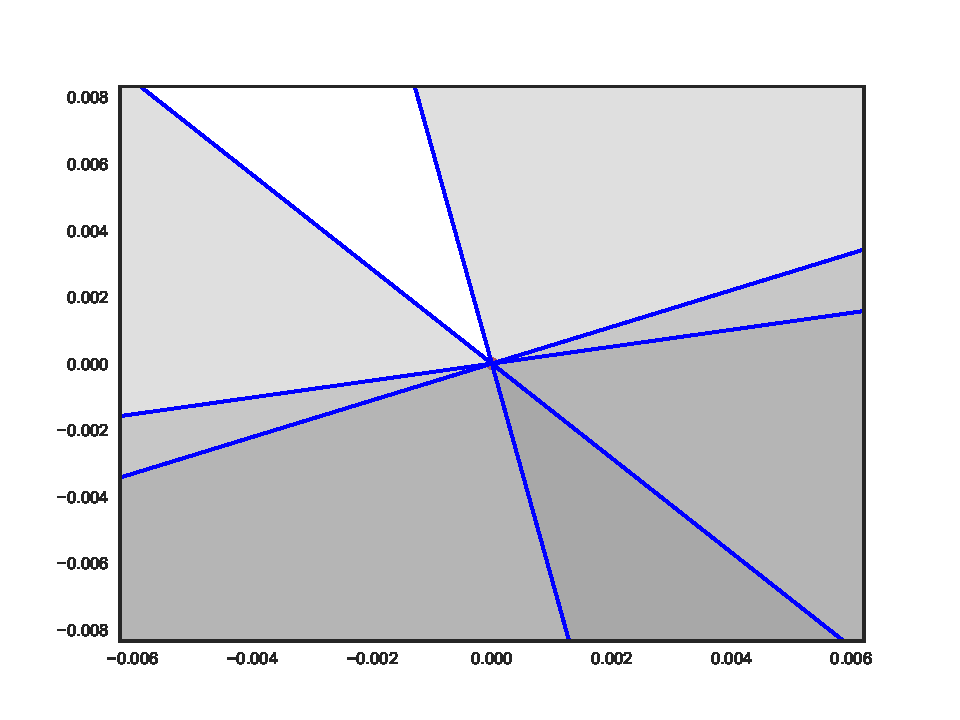
\includegraphics[width=\hsize]{img/toy/relu/conv2d_25-2.pdf}}
    }
    % \hskip1em
    \parbox{.195\textwidth}{%
      \subcaptionbox{Feature layer\label{fig:moonsReLUFeature1}}{\includegraphics[width=\hsize]{img/toy/relu/dense_1-0.pdf}}
    %   \vskip1em
      \subcaptionbox{Feature layer\label{fig:moonsReLUFeature2}}{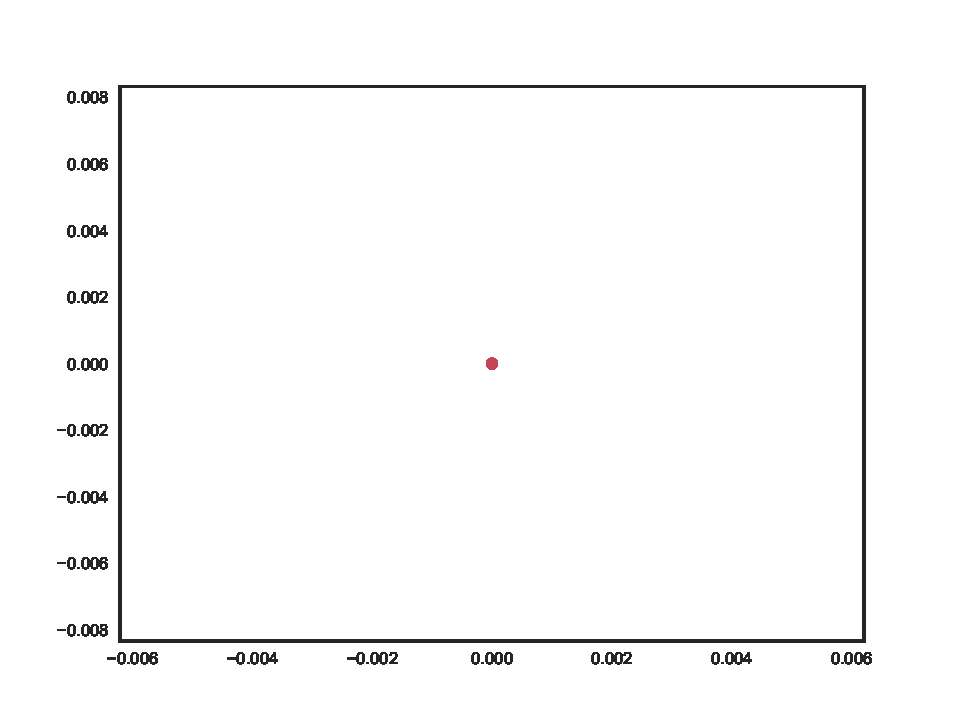
\includegraphics[width=\hsize]{img/toy/relu/dense_1-2.pdf}}
    }
    % \hskip1em
    \parbox{.195\textwidth}{%
      \subcaptionbox{Output\label{fig:moonsReLUOutput}}{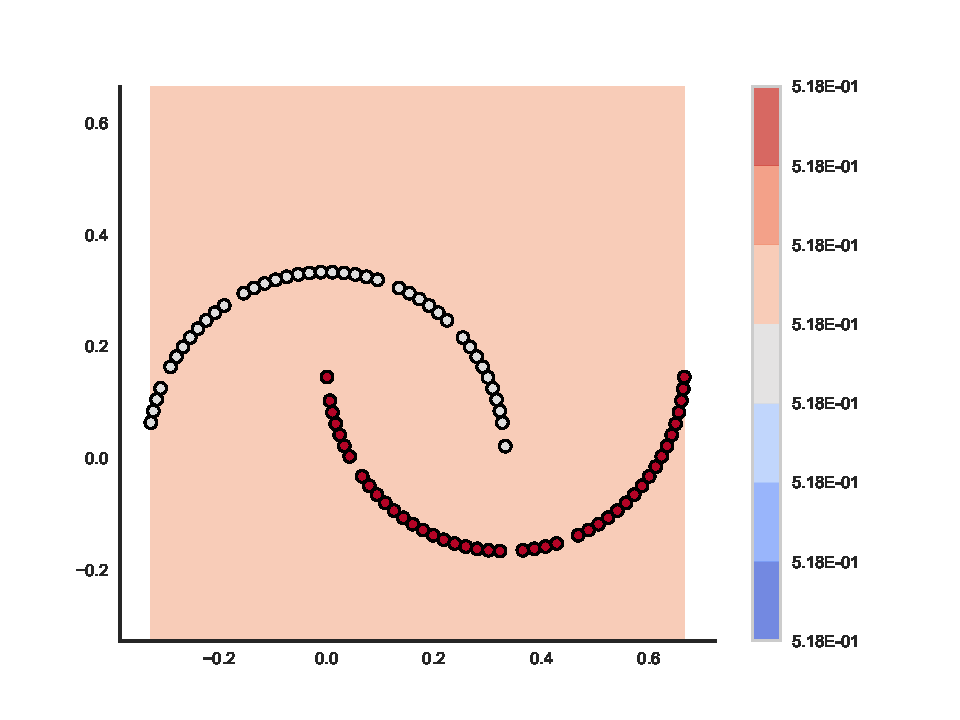
\includegraphics[clip, trim=2.35cm 1.75cm 4.5cm 0cm,width=\hsize]{img/toy/relu/output.pdf}}
    }
  }
  \caption{Data transformed across a 50x4 \ReLU classification network. Notice how the the dataset is progressively mapped to zero as it traverses the network. This renders the output layer unable to solve the problem.}
    \label{fig:moonsReLU}
\end{figure*}

\begin{figure*}[h!]
  \centering
  \parbox{\textwidth}{
    \parbox{.195\textwidth}{%
      \subcaptionbox{Input layer\label{fig:moonsReLUBNInput}}{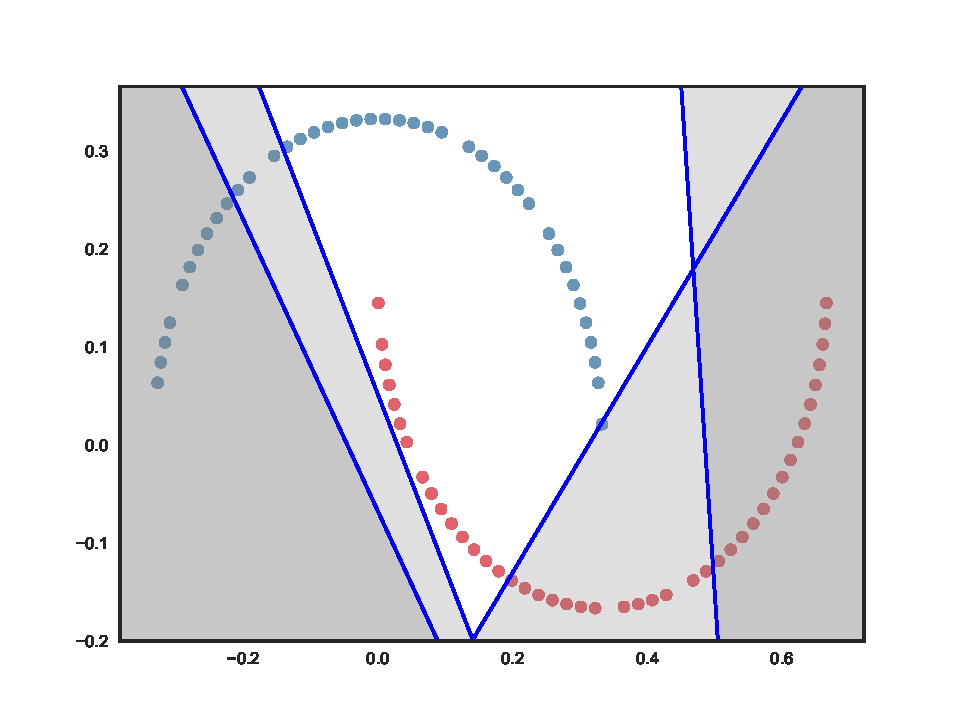
\includegraphics[width=\hsize]{img/toy/relu-bn/conv2d_1-0.pdf}}
    }
    % \hskip1em
    \parbox{.195\textwidth}{%
      \subcaptionbox{4th layer\label{fig:moonsReLUBN41}}{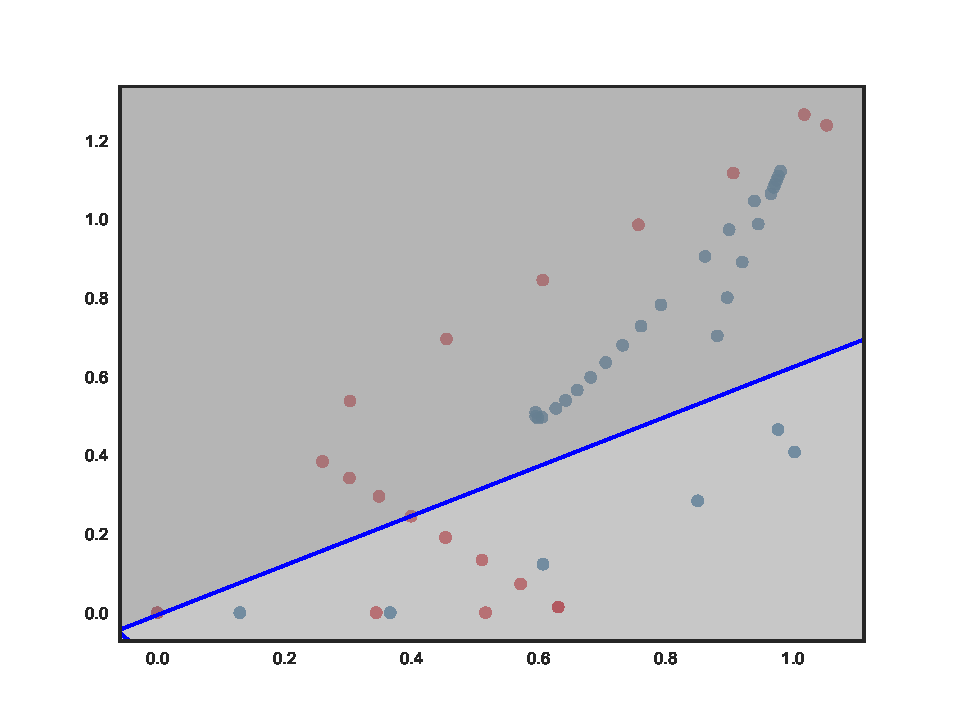
\includegraphics[width=\hsize]{img/toy/relu-bn/conv2d_4-0.pdf}}
    %   \vskip1em
      \subcaptionbox{4th layer\label{fig:moonsReLUBN42}}{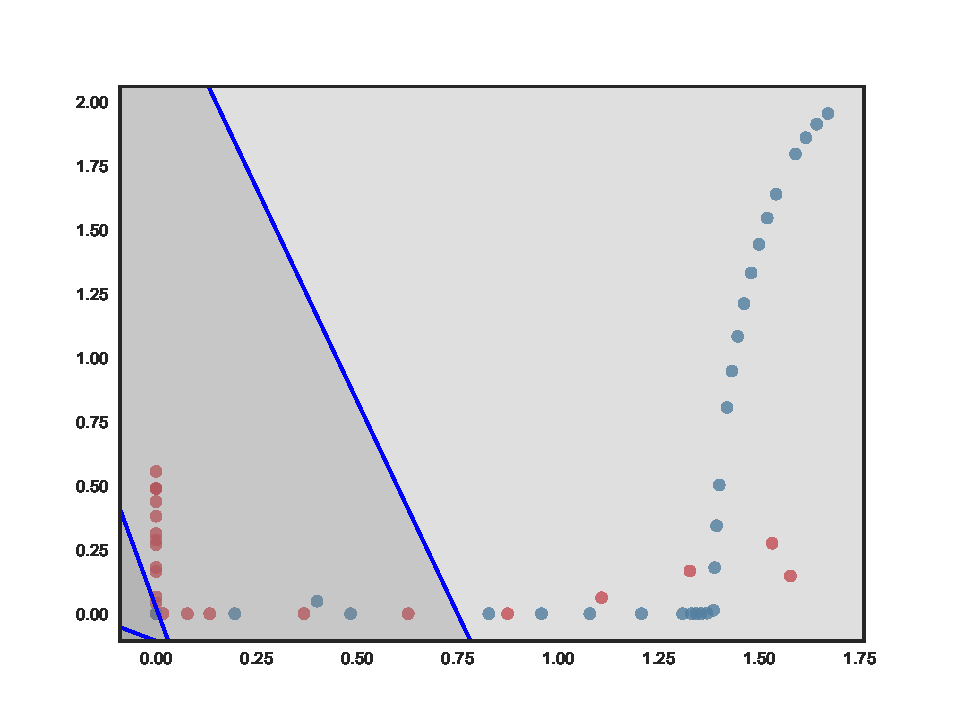
\includegraphics[width=\hsize]{img/toy/relu-bn/conv2d_4-2.pdf}}
    }
    % \hskip1em
    \parbox{.195\textwidth}{%
      \subcaptionbox{25th layer\label{fig:moonsReLUBN251}}{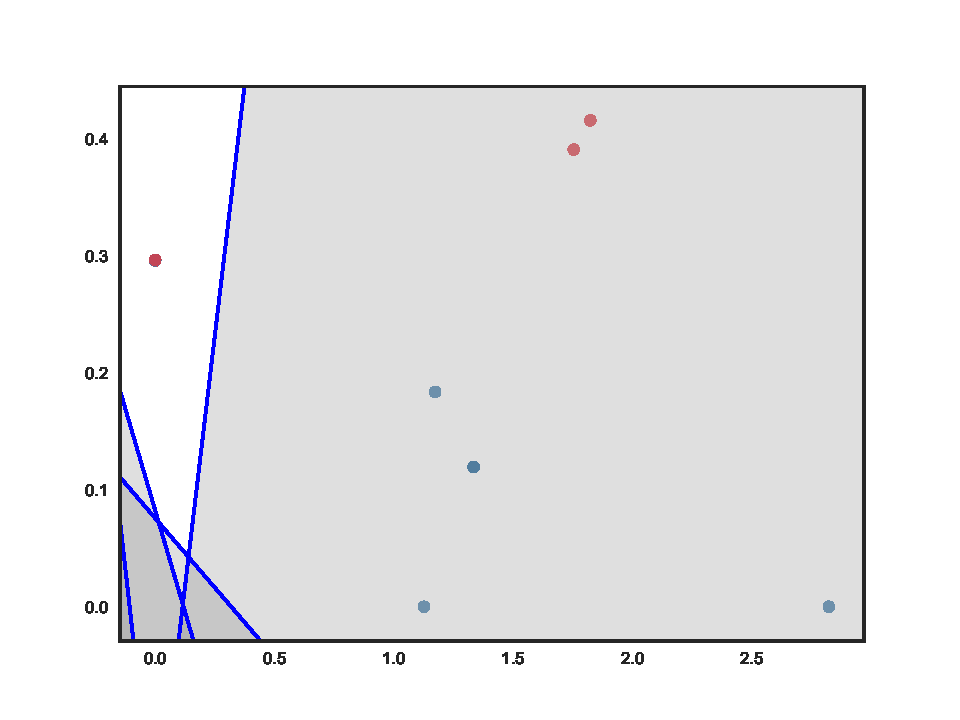
\includegraphics[width=\hsize]{img/toy/relu-bn/conv2d_25-0.pdf}}
    %   \vskip1em
      \subcaptionbox{25th layer\label{fig:moonsReLUBN252}}{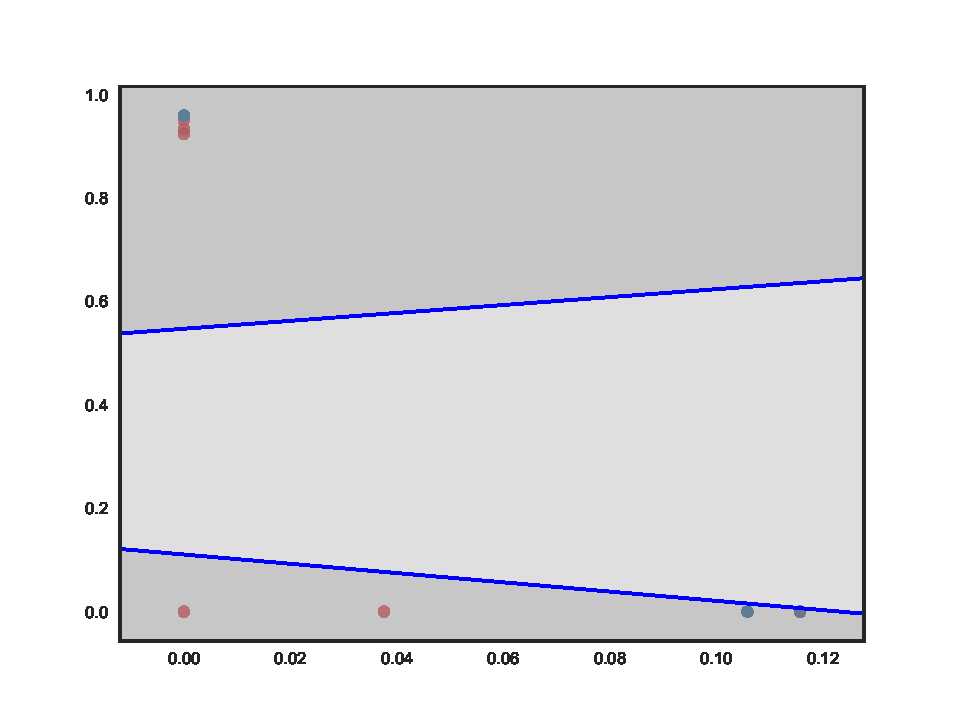
\includegraphics[width=\hsize]{img/toy/relu-bn/conv2d_25-2.pdf}} 
    }
    % \hskip1em
    \parbox{.195\textwidth}{%
      \subcaptionbox{Feature layer\label{fig:moonsReLUBNFeature1}}{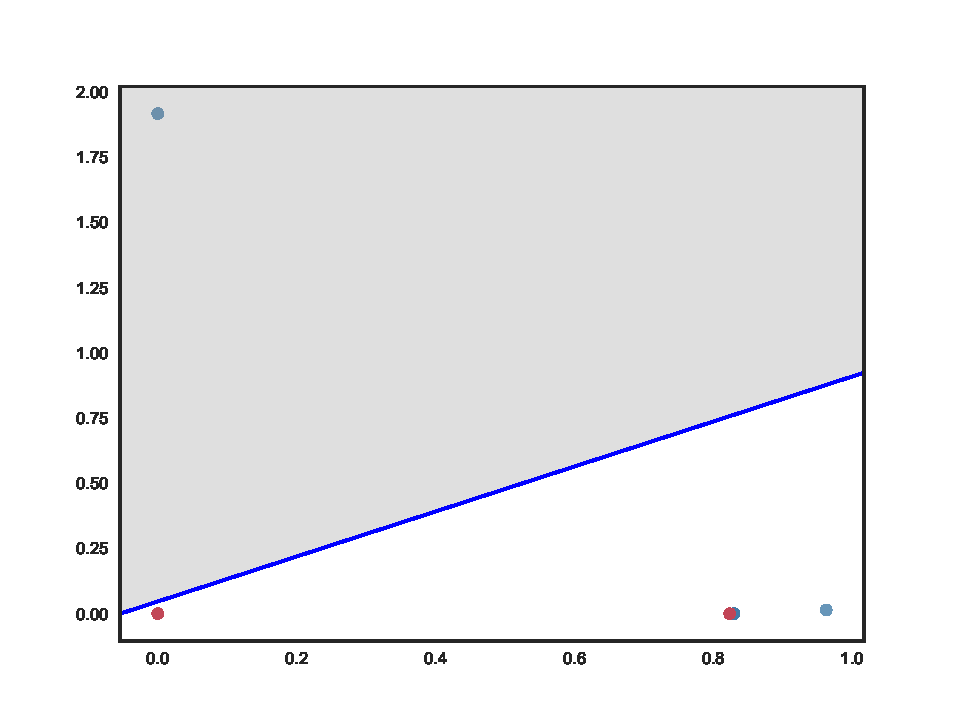
\includegraphics[width=\hsize]{img/toy/relu-bn/dense_1-0.pdf}}
    %   \vskip1em
      \subcaptionbox{Feature layer\label{fig:moonsReLUBNFeature2}}{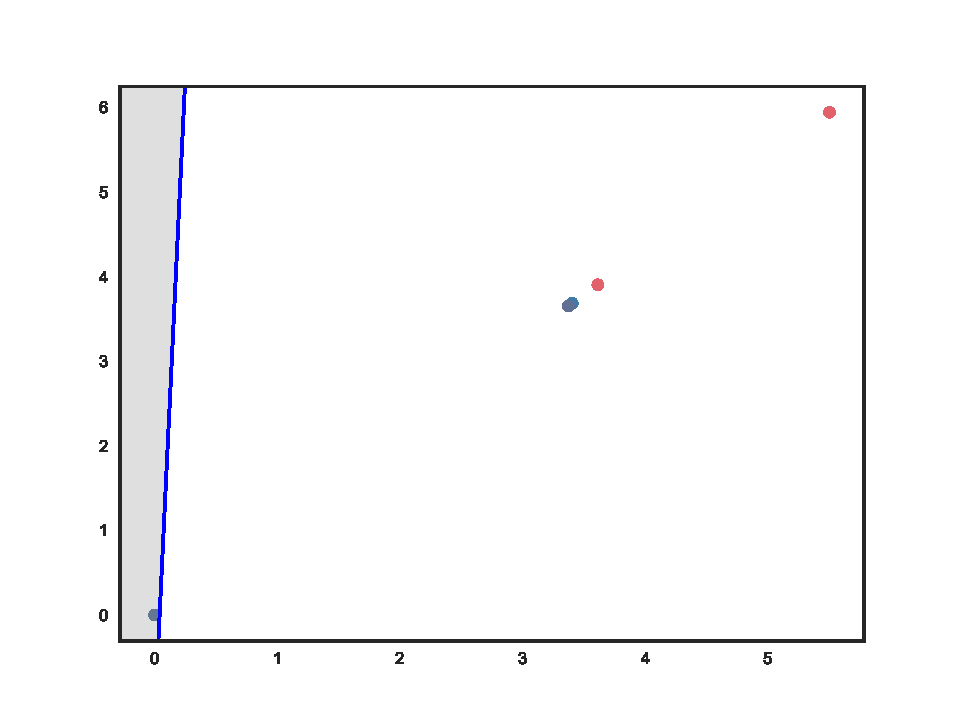
\includegraphics[width=\hsize]{img/toy/relu-bn/dense_1-2.pdf}} 
    }
    % \hskip1em
    \parbox{.195\textwidth}{%
      \subcaptionbox{Output\label{fig:moonsReLUBNOutput}}{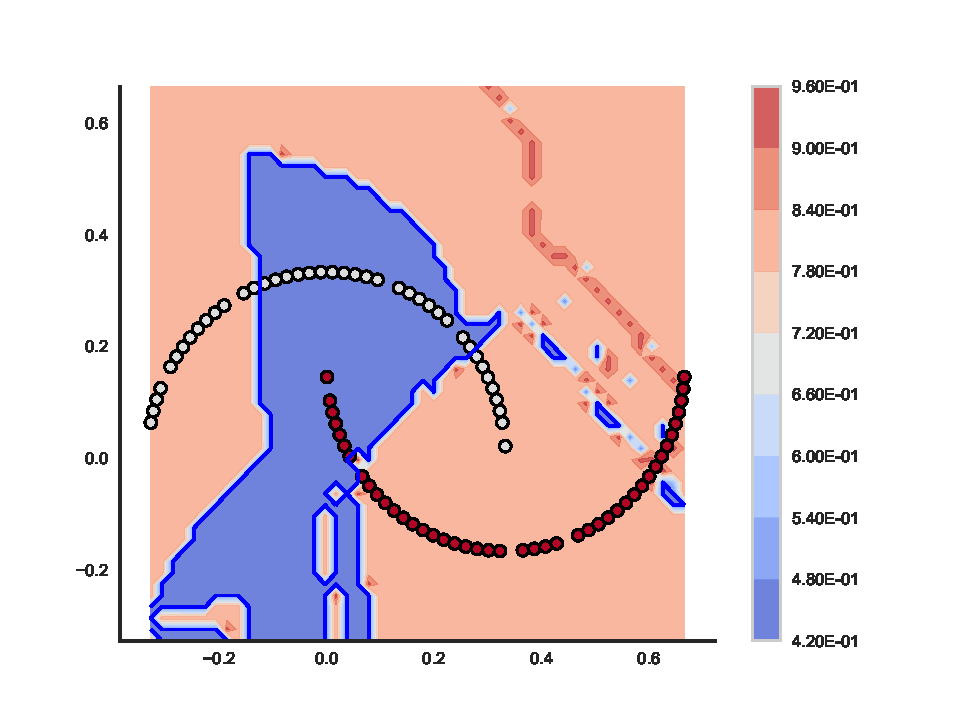
\includegraphics[clip, trim=2.35cm 1.75cm 4.5cm 0cm,width=\hsize]{img/toy/relu-bn/output.pdf}}
    }
  }
  \caption{Data transformed across a 50x4 \ReLUBN network. The dataset is collapsed in few points at the feature layer. As the gradient cannot be backpropagated across the truncation after the affine transform of $\gamma$ and $\beta$ despite the standarization, failing in the same manner than \ReLU only that with non-zero activations. This results in \emph{topological mixing} of the datasets. Therefore, the representational capability of the network is hindered to such extent that the resulting output, although non-trivial, is totally arbitrary.}
    \label{fig:moonsReLUBN}
\end{figure*}


\begin{figure*}[h!]
  \centering
     % Unitwise
  \parbox{\textwidth}{
    \parbox{.195\textwidth}{%
      \subcaptionbox{Input layer\label{fig:moonsUnitwiseInput}}{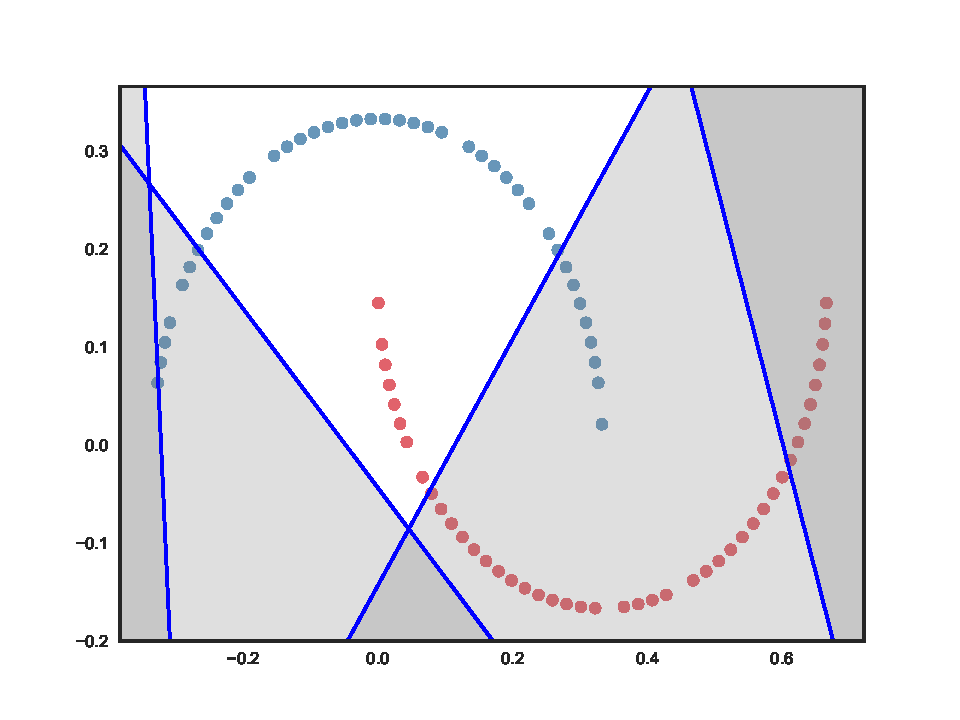
\includegraphics[width=\hsize]{img/toy/unitwise/conv2d_1-0.pdf}}
    }
    % \hskip1em
    \parbox{.195\textwidth}{%
      \subcaptionbox{4th layer\label{fig:moonsUnitwise41}}{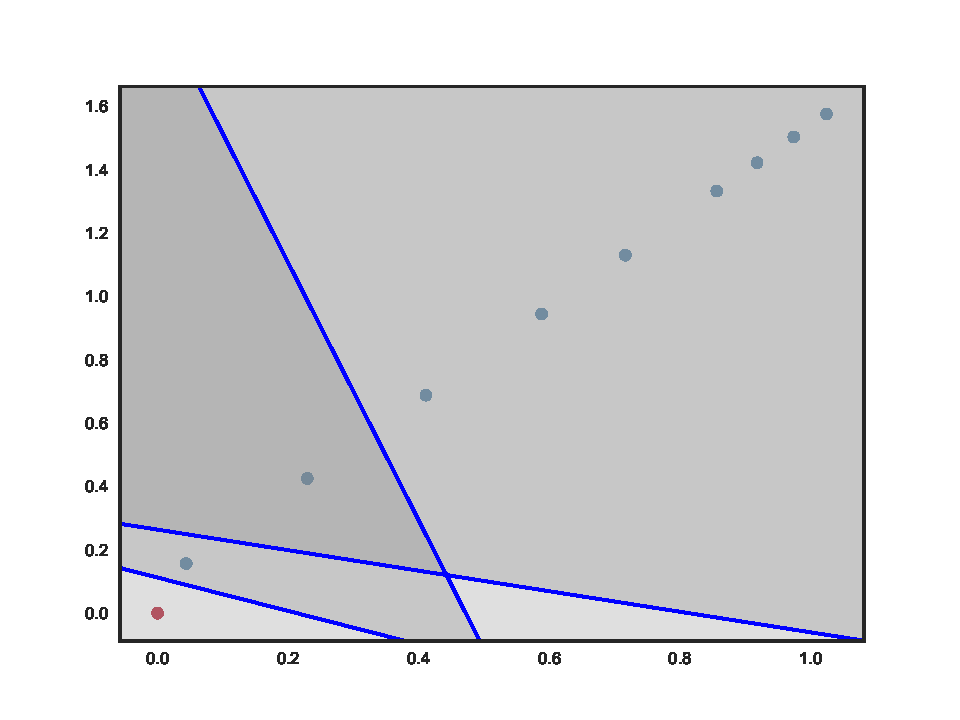
\includegraphics[width=\hsize]{img/toy/unitwise/conv2d_4-0.pdf}}
    %   \vskip1em
      \subcaptionbox{4th layer\label{fig:moonsUnitwise42}}{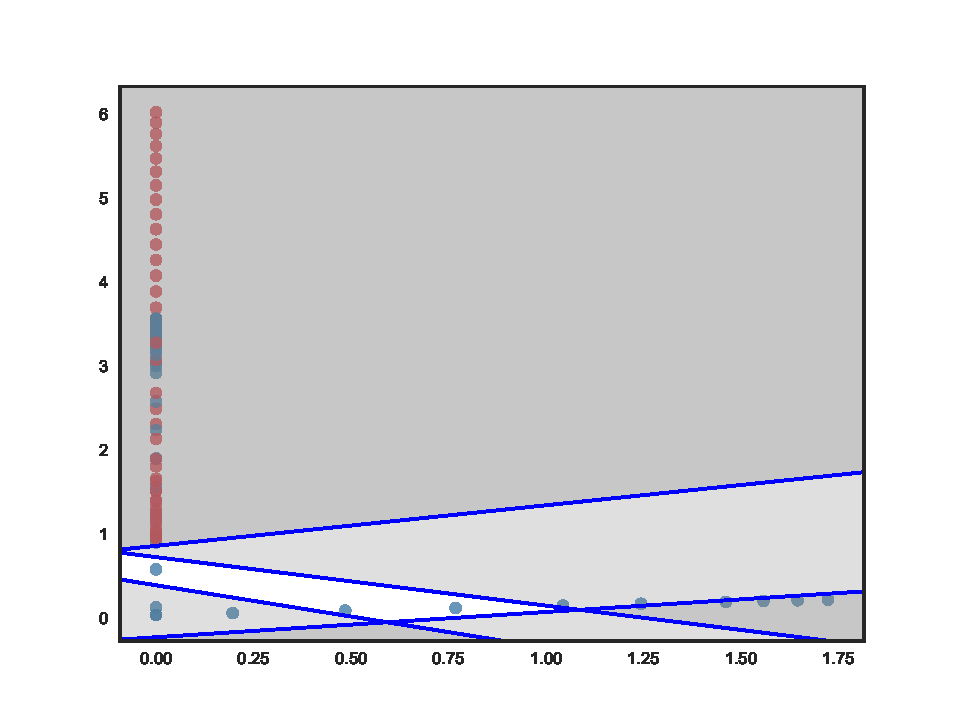
\includegraphics[width=\hsize]{img/toy/unitwise/conv2d_4-2.pdf}}
    }
    % \hskip1em
    \parbox{.195\textwidth}{%
      \subcaptionbox{25th layer\label{fig:moonsUnitwise251}}{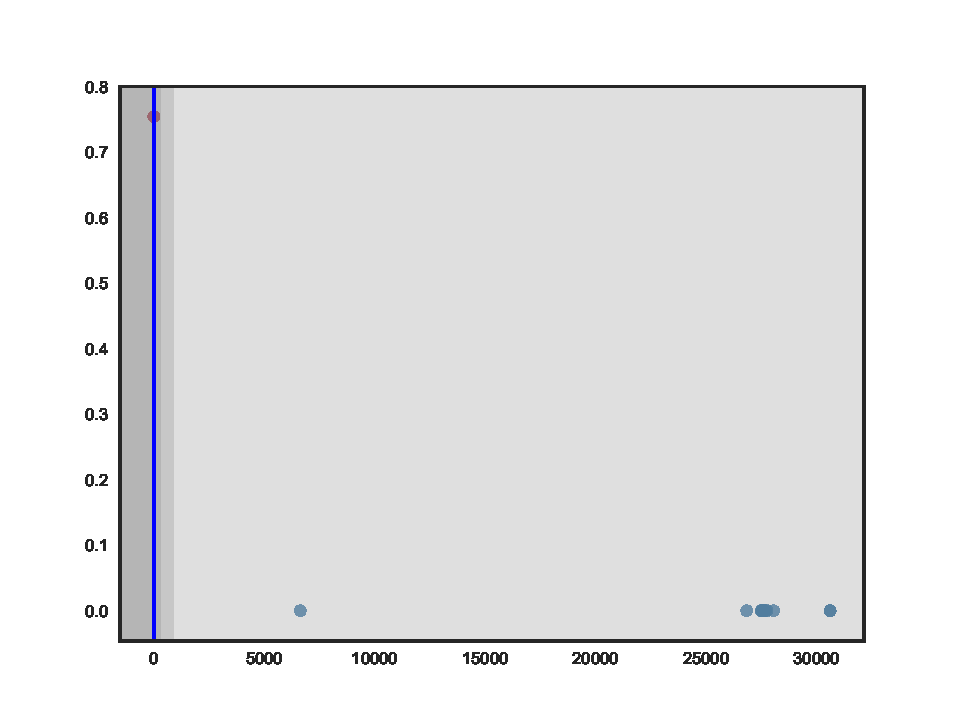
\includegraphics[width=\hsize]{img/toy/unitwise/conv2d_25-0.pdf}}
    %   \vskip1em
      \subcaptionbox{25th layer\label{fig:moonsUnitwise252}}{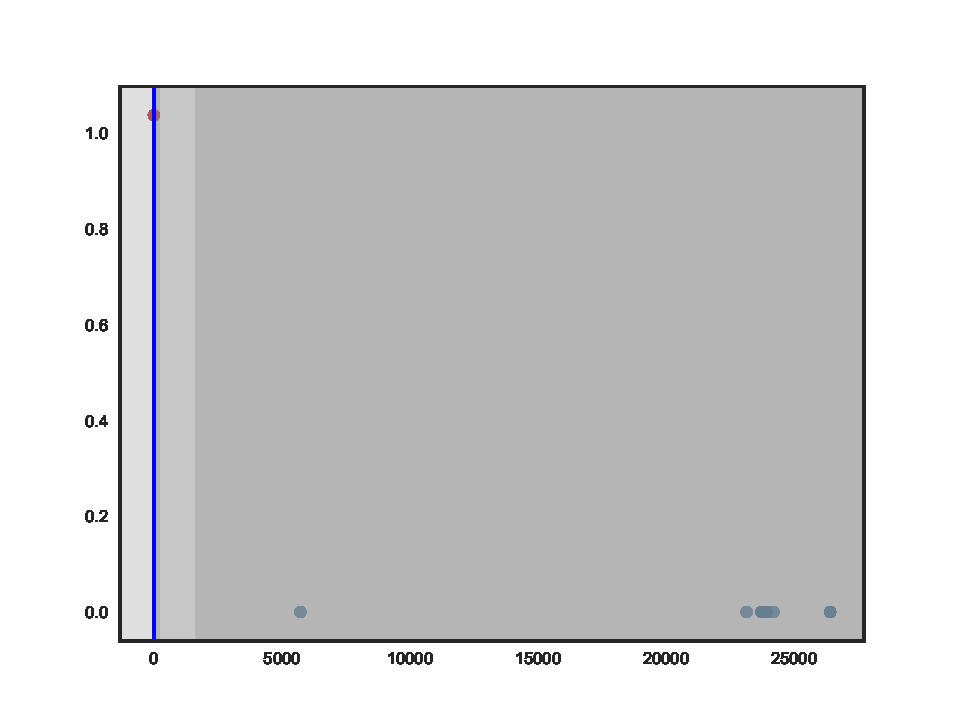
\includegraphics[width=\hsize]{img/toy/unitwise/conv2d_25-2.pdf}}
    }
    % \hskip1em
    \parbox{.195\textwidth}{%
      \subcaptionbox{Feature layer\label{fig:moonsUnitwiseFeature1}}{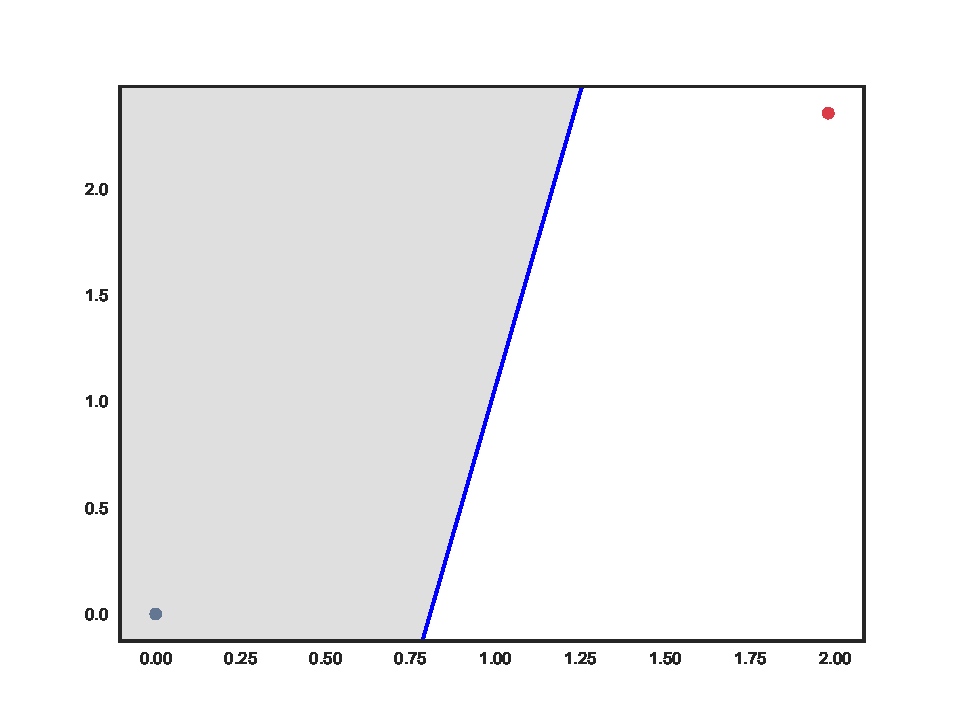
\includegraphics[width=\hsize]{img/toy/unitwise/dense_1-0.pdf}}
    %   \vskip1em
      \subcaptionbox{Feature layer\label{fig:moonsUnitwiseFeature2}}{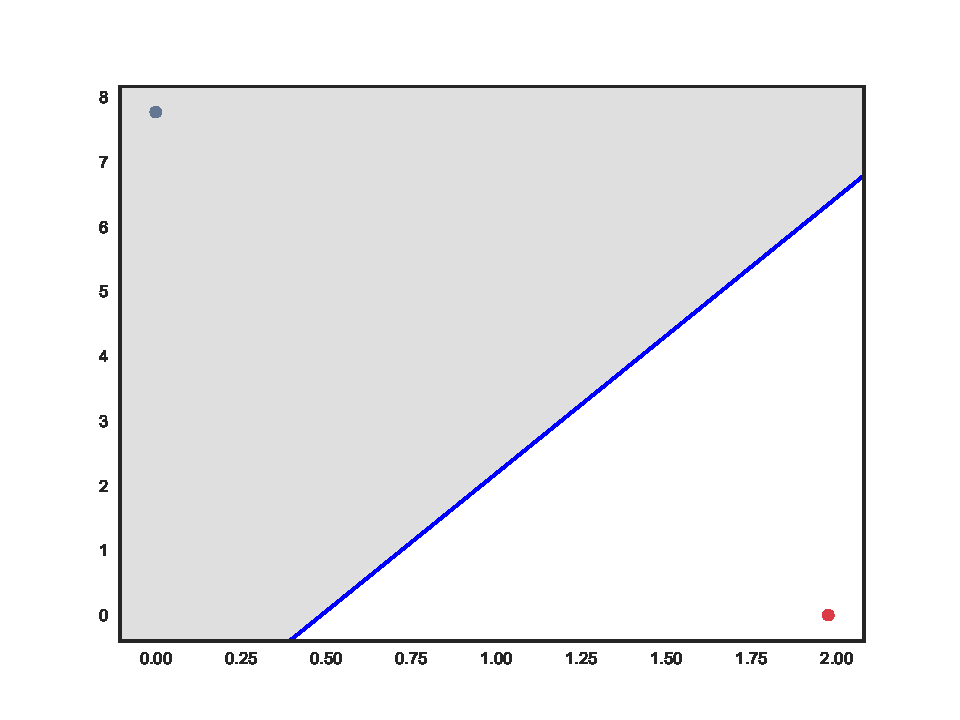
\includegraphics[width=\hsize]{img/toy/unitwise/dense_1-2.pdf}}
    }
    % \hskip1em
    \parbox{.195\textwidth}{%
      \subcaptionbox{Output\label{fig:moonsUnitwiseOutput}}{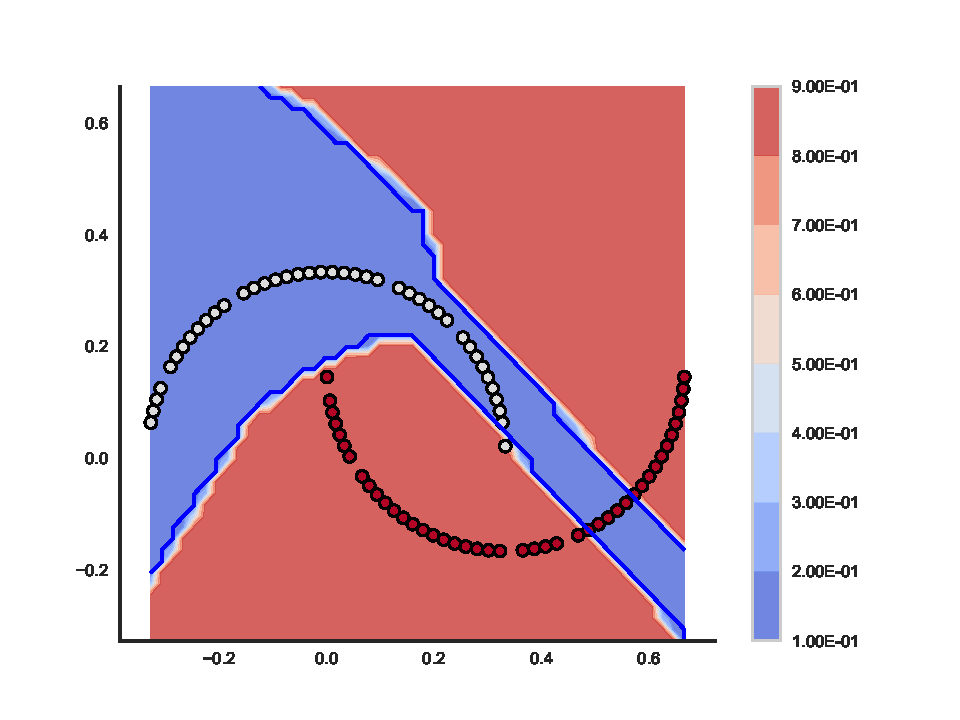
\includegraphics[clip, trim=2.35cm 1.75cm 4.5cm 0cm,width=\hsize]{img/toy/unitwise/output.pdf}}
    }
  }
  \caption{Data transformed across a 50x4 \SepUnit network. Notice how dead and affine units have been reduced. Despite collapsing the dataset in two points at the feature layer, the classification performed in the output layer is approximately correct. We conjecture that this is due the dead point addressed with \SepPoint.}
    \label{fig:moonsUnitwise}
\end{figure*}



\begin{figure*}[h!]
  \centering
  %Pointwise
  \parbox{\textwidth}{
    \parbox{.195\textwidth}{%
      \subcaptionbox{Input layer\label{fig:moonsPointwiseInput}}{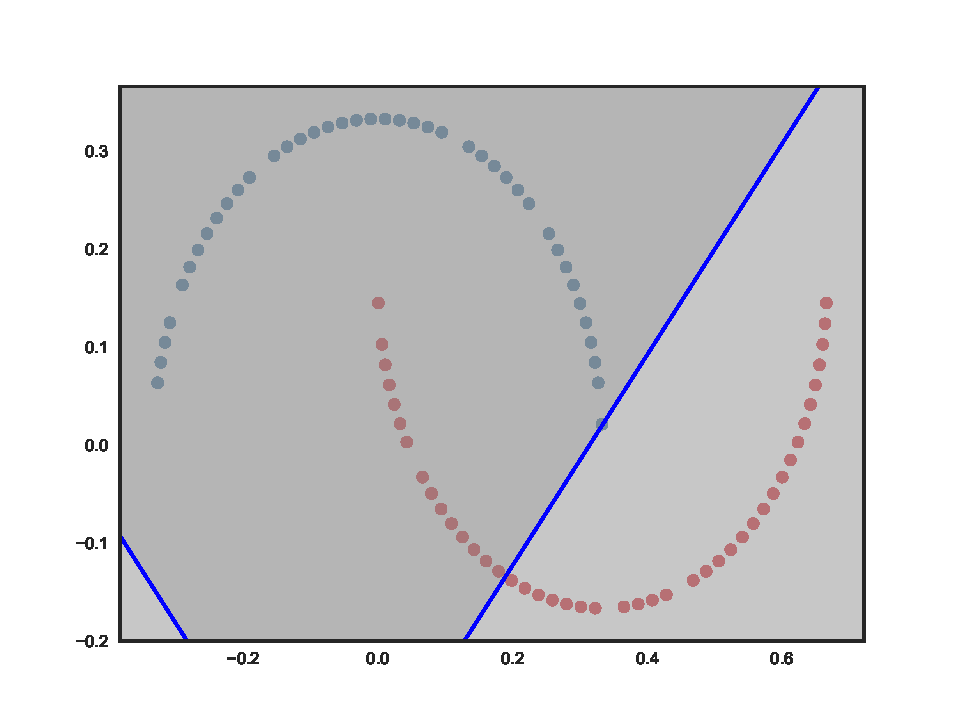
\includegraphics[width=\hsize]{img/toy/pointwise/conv2d_1-0.pdf}}
    }
    % \hskip1em
    \parbox{.195\textwidth}{%
      \subcaptionbox{4th layer\label{fig:moonsPointwise41}}{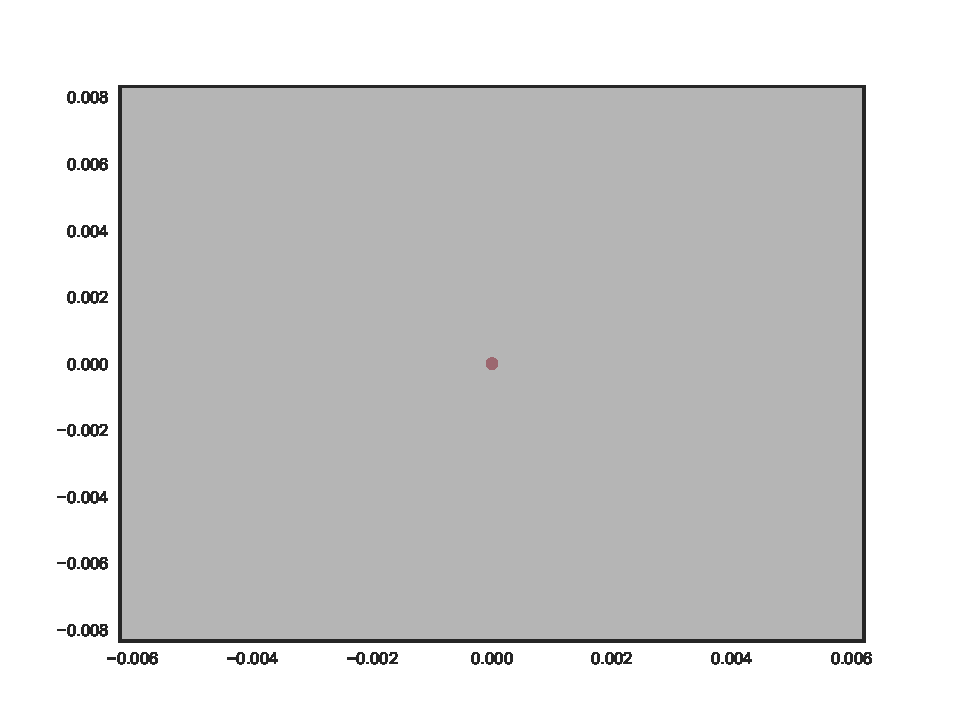
\includegraphics[width=\hsize]{img/toy/pointwise/conv2d_4-0.pdf}}
    %   \vskip1em
      \subcaptionbox{4th layer\label{fig:moonsPointwise42}}{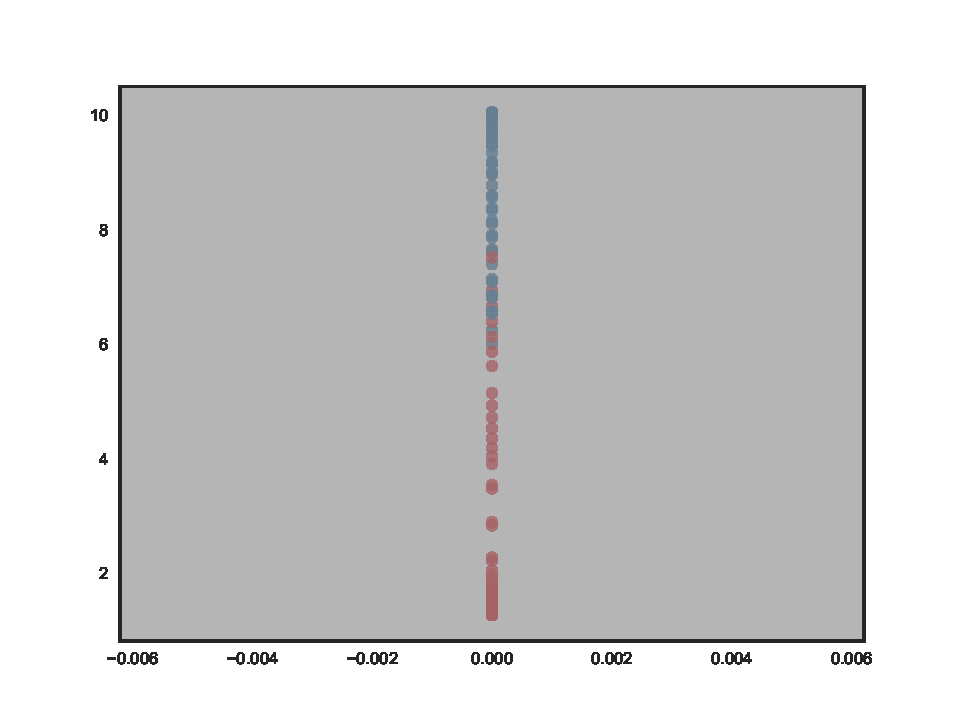
\includegraphics[width=\hsize]{img/toy/pointwise/conv2d_4-2.pdf}} 
    }
    % \hskip1em
    \parbox{.195\textwidth}{%
      \subcaptionbox{25th layer\label{fig:moonsPointwise251}}{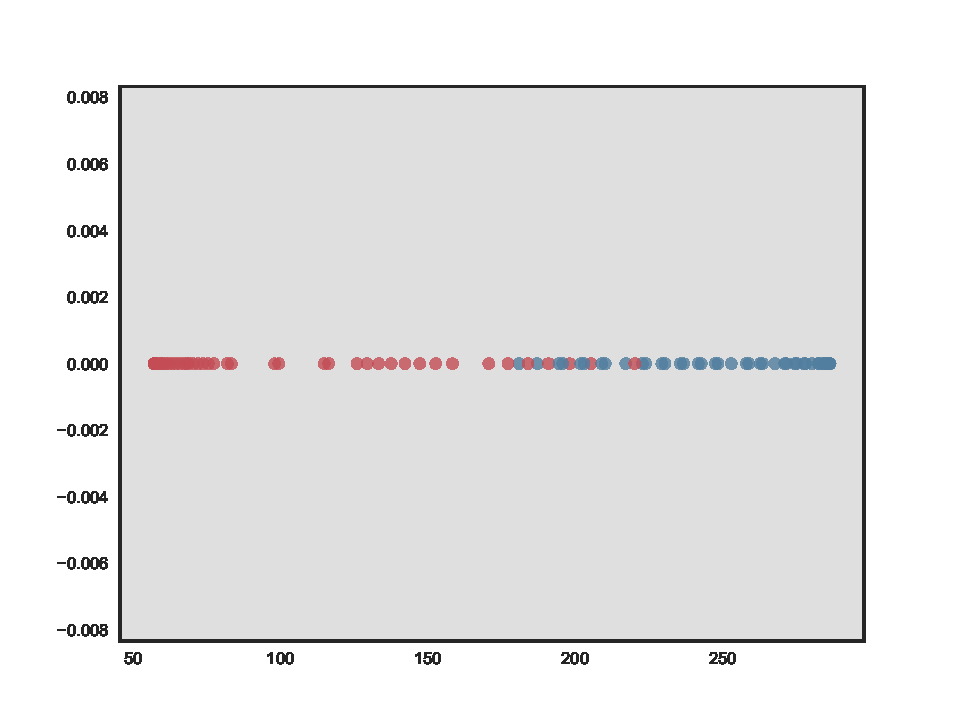
\includegraphics[width=\hsize]{img/toy/pointwise/conv2d_25-0.pdf}}
    %   \vskip1em
      \subcaptionbox{25th layer\label{fig:moonsPointwise252}}{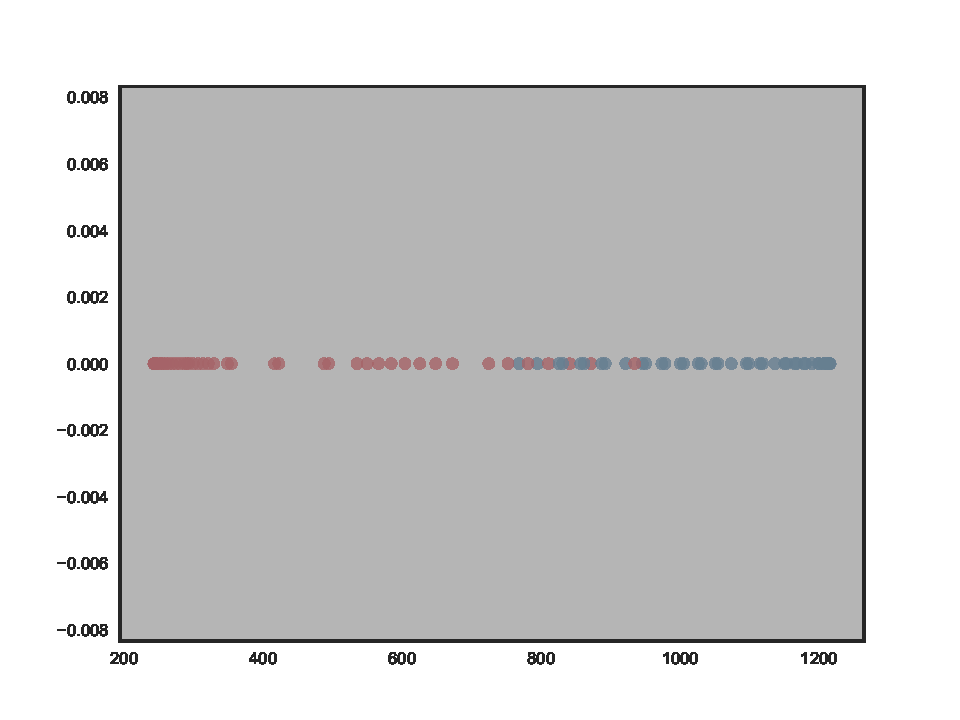
\includegraphics[width=\hsize]{img/toy/pointwise/conv2d_25-2.pdf}} 
    }
    % \hskip1em
    \parbox{.195\textwidth}{%
      \subcaptionbox{Feature layer\label{fig:moonsPointwiseFeature1}}{\includegraphics[width=\hsize]{img/toy/pointwise/dense_1-0.pdf}}
    %   \vskip1em
      \subcaptionbox{Feature layer\label{fig:moonsPointwiseFeature2}}{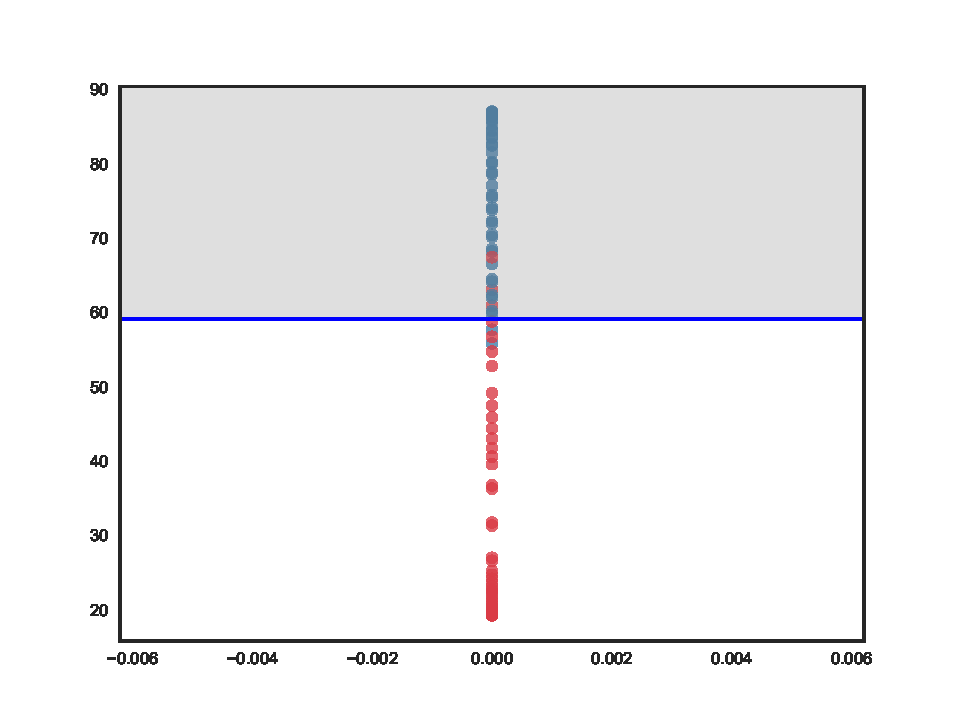
\includegraphics[width=\hsize]{img/toy/pointwise/dense_1-2.pdf}} 
    }
    % \hskip1em
    \parbox{.195\textwidth}{%
      \subcaptionbox{Output\label{fig:moonsPointwiseOutput}}{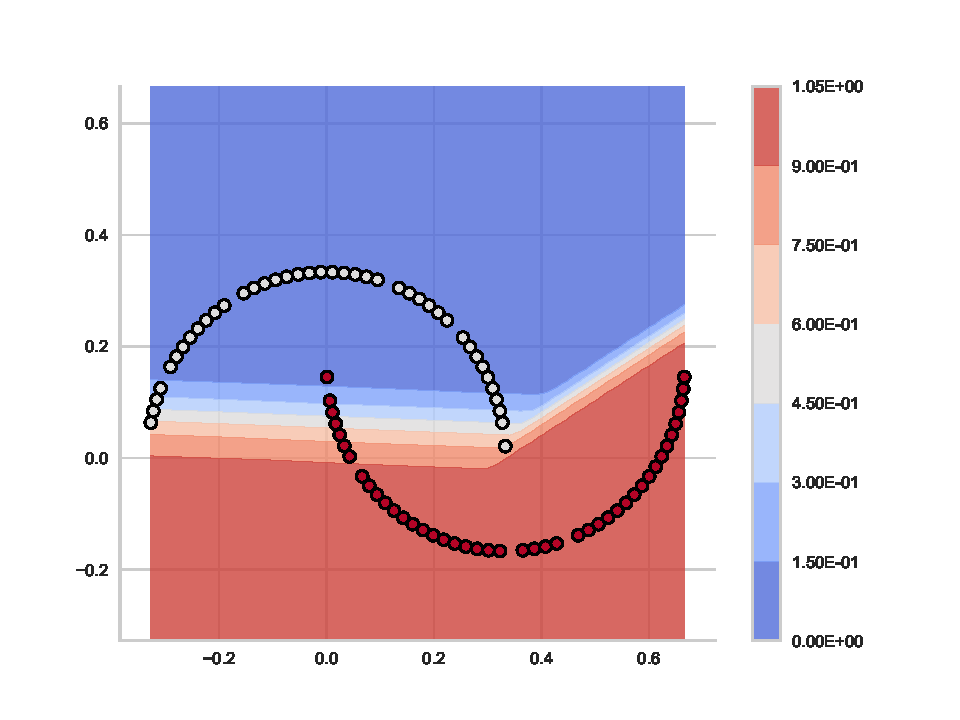
\includegraphics[clip, trim=2.35cm 1.75cm 4.5cm 0cm,width=\hsize]{img/toy/pointwise/output.pdf}}
    }
  }
  \caption{Data transformed across a 50x4 \SepPoint network. The network displays a richer internal representation without collapsing the dataset like \SepUnit or \ReLUBN. However, plenty of dead and affine units appear since they are not penalized, causing underfitting.}
    \label{fig:moonsPointwise}
\end{figure*}


\begin{figure*}[h!]
  \centering
   \parbox{\textwidth}{
    \parbox{.195\textwidth}{%
      \subcaptionbox{Input layer\label{fig:moonsUnitpointwiseInput}}{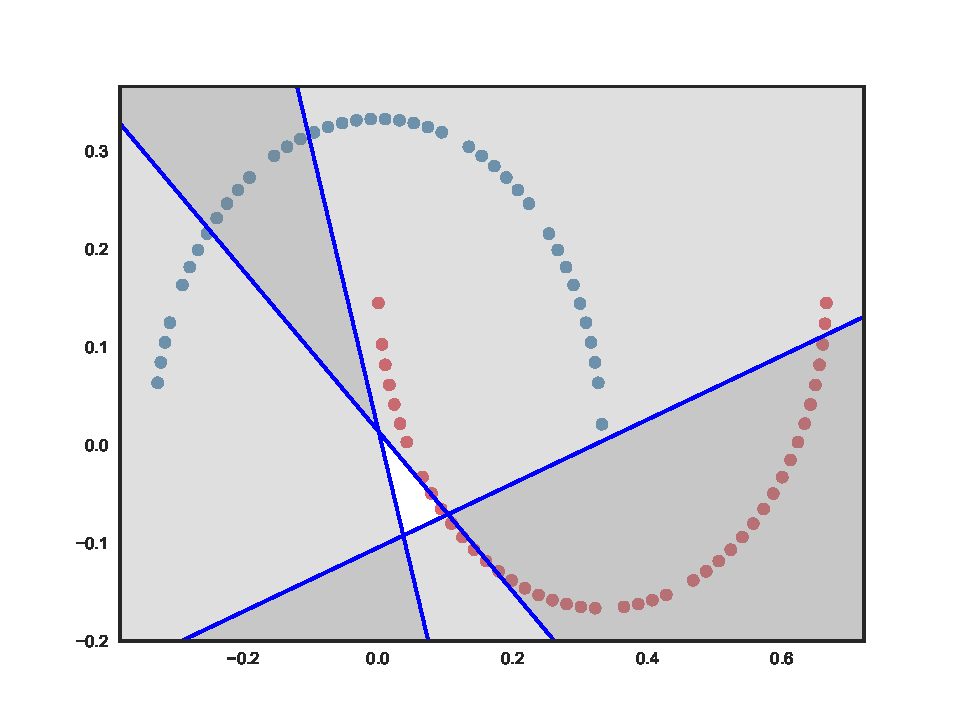
\includegraphics[width=\hsize]{img/toy/unitpointwise/conv2d_1-0.pdf}}
    }
    % \hskip1em
    \parbox{.195\textwidth}{%
      \subcaptionbox{4th layer\label{fig:moonsUnitpointwise41}}{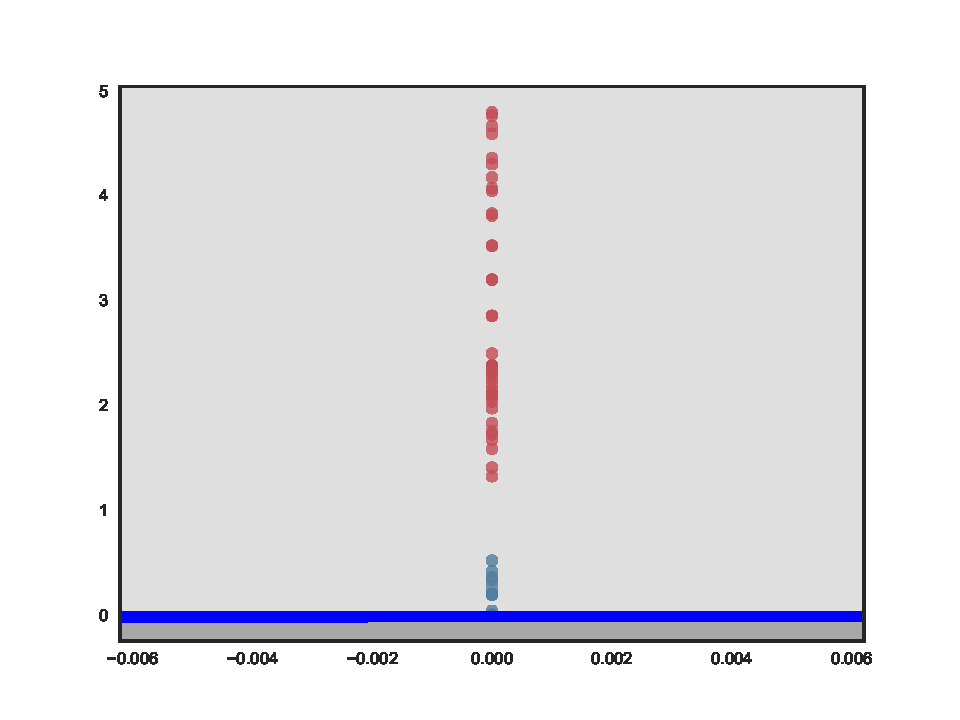
\includegraphics[width=\hsize]{img/toy/unitpointwise/conv2d_4-0.pdf}}
    %   \vskip1em
      \subcaptionbox{4th layer\label{fig:moonsUnitpointwise42}}{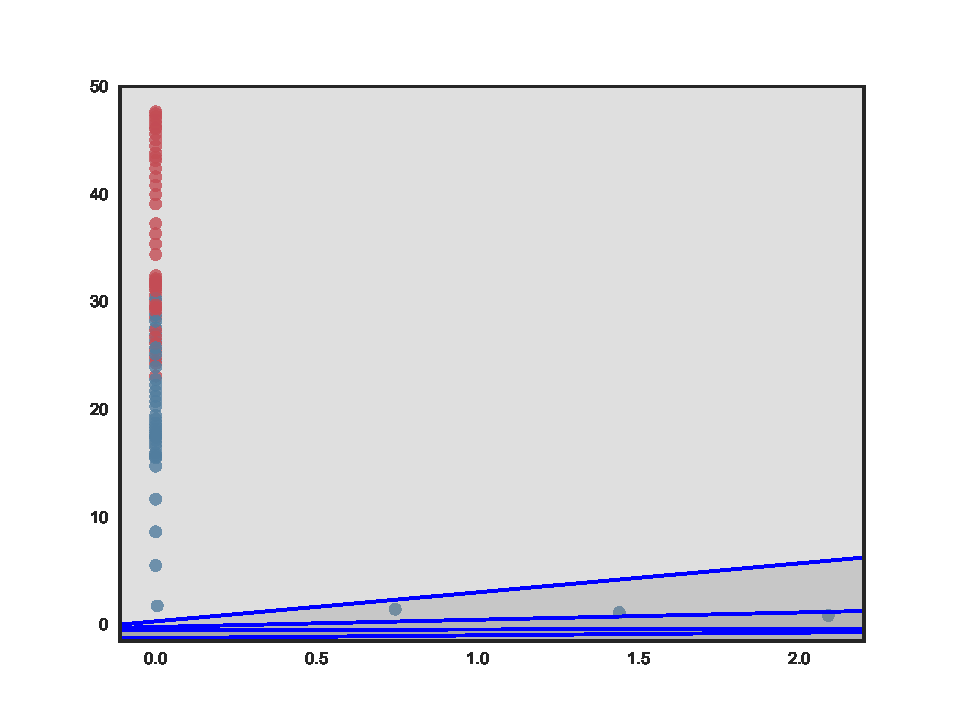
\includegraphics[width=\hsize]{img/toy/unitpointwise/conv2d_4-2.pdf}} 
    }
    % \hskip1em
    \parbox{.195\textwidth}{%
      \subcaptionbox{25th layer\label{fig:moonsUnitpointwise251}}{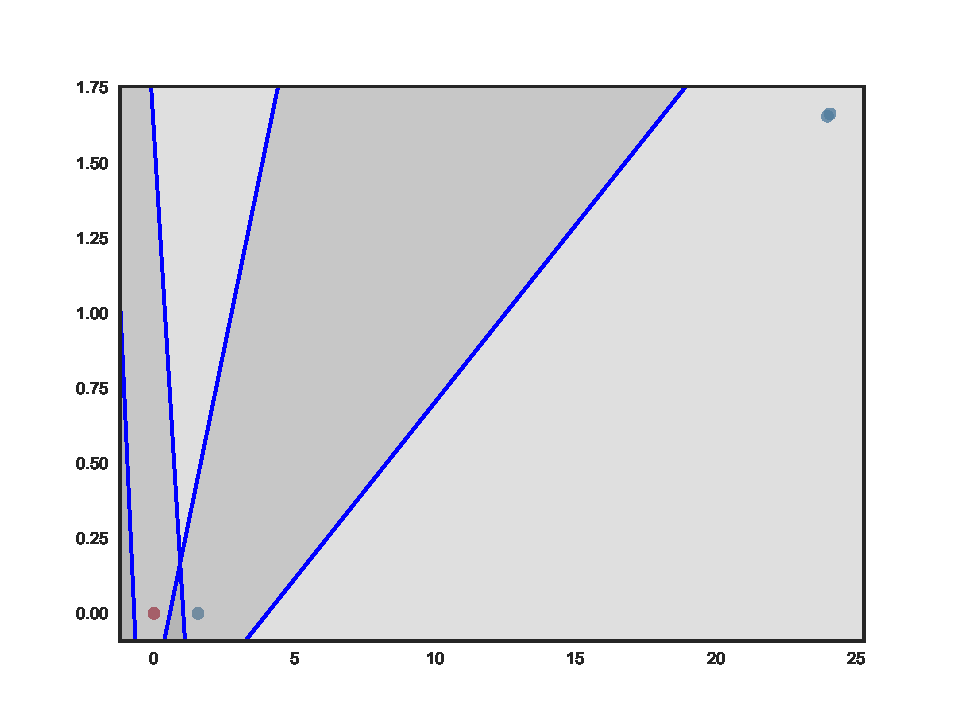
\includegraphics[width=\hsize]{img/toy/unitpointwise/conv2d_25-0.pdf}}
    %   \vskip1em
      \subcaptionbox{25th layer\label{fig:moonsUnitpointwise252}}{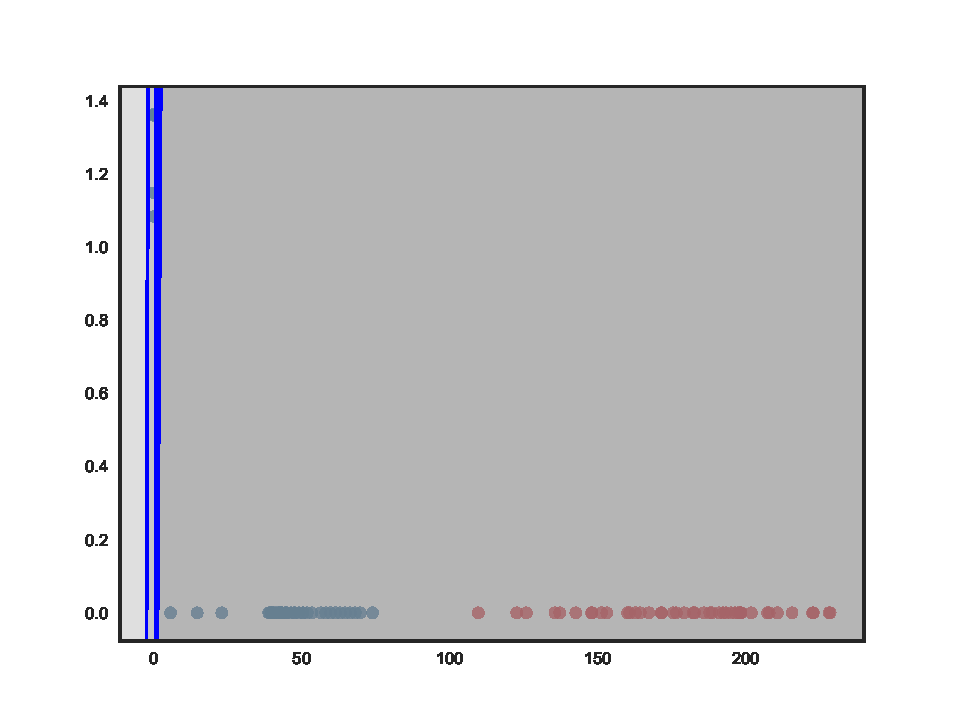
\includegraphics[width=\hsize]{img/toy/unitpointwise/conv2d_25-2.pdf}} 
    }
    % \hskip1em
    \parbox{.195\textwidth}{%
      \subcaptionbox{Feature layer\label{fig:moonsUnitpointwiseFeature1}}{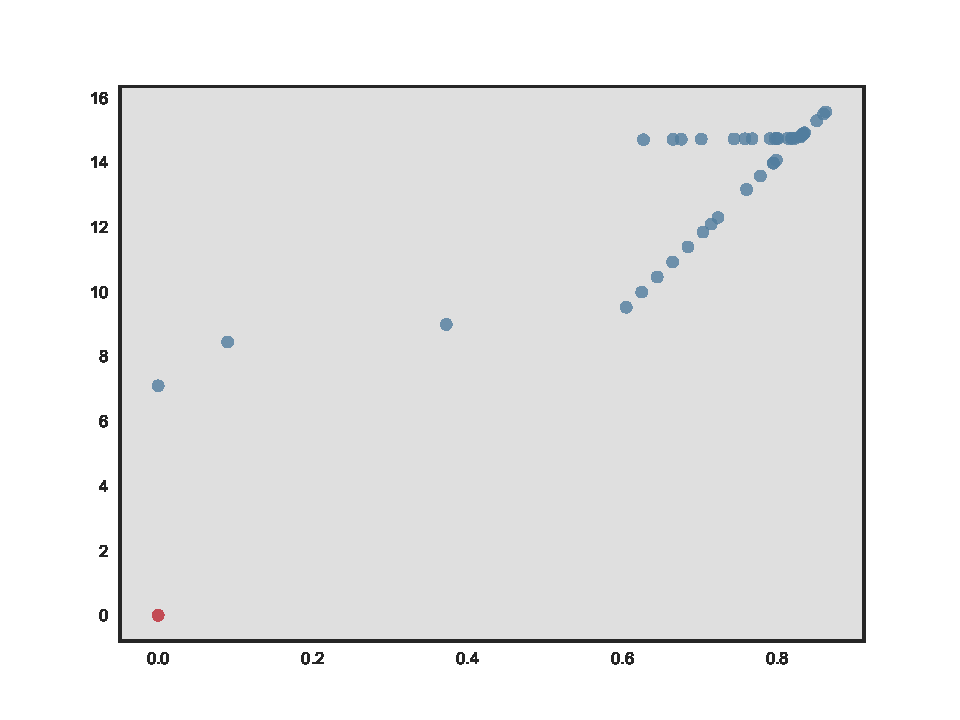
\includegraphics[width=\hsize]{img/toy/unitpointwise/dense_1-0.pdf}}
    %   \vskip1em
      \subcaptionbox{Feature layer\label{fig:moonsUnitpointwiseFeature2}}{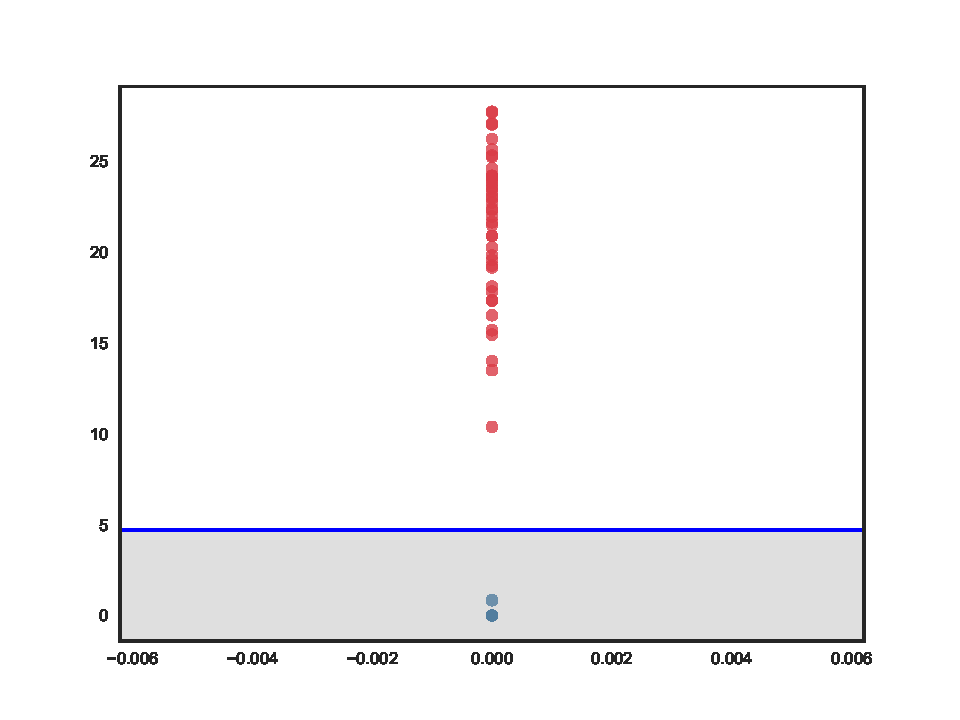
\includegraphics[width=\hsize]{img/toy/unitpointwise/dense_1-2.pdf}} 
    }
    % \hskip1em
    \parbox{.195\textwidth}{%
      \subcaptionbox{Output\label{fig:moonsUnitpointwiseOutput}}{
      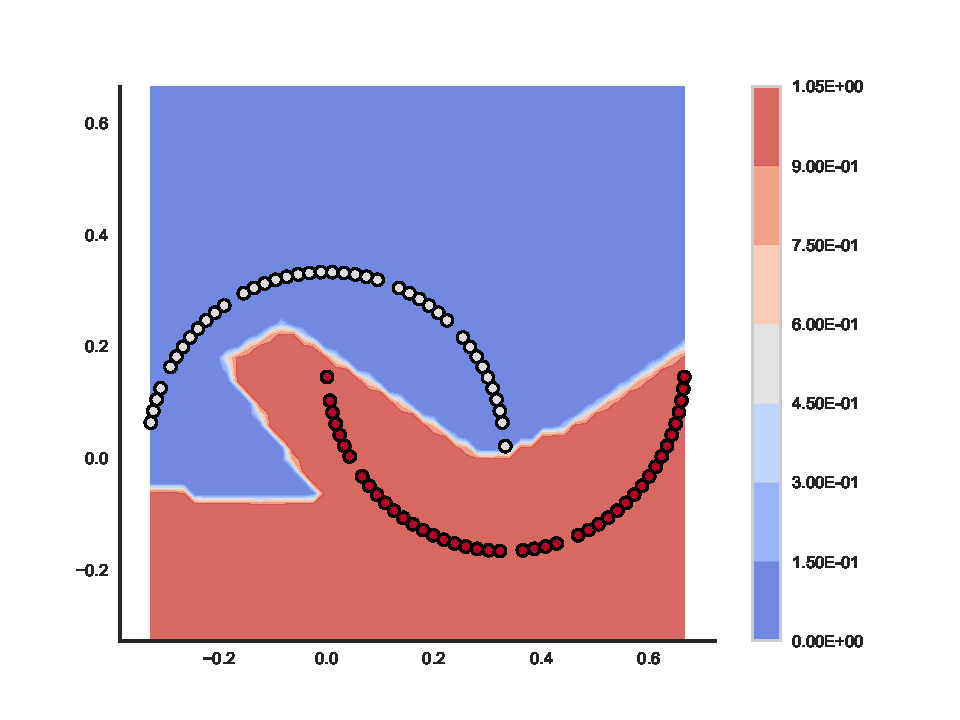
\includegraphics[clip, trim=2.35cm 1.75cm 4.5cm 0cm,width=\hsize, height=\hsize]{img/toy/unitpointwise/output.pdf}
      }
    }
  }

    \caption{Data transformed across a 50x4 \SepUnitPoint network. The network displays internal representations without collapsing the dataset like \SepPoint while retaining classification power like \SepUnit.}
    \label{fig:moonsUnitPointwise}
\end{figure*}

\begin{figure*}[h!]
  \centering
  \parbox{\textwidth}{
    \parbox{.195\textwidth}{%
      \subcaptionbox{Input layer\label{fig:moonsLayerwiseInput}}{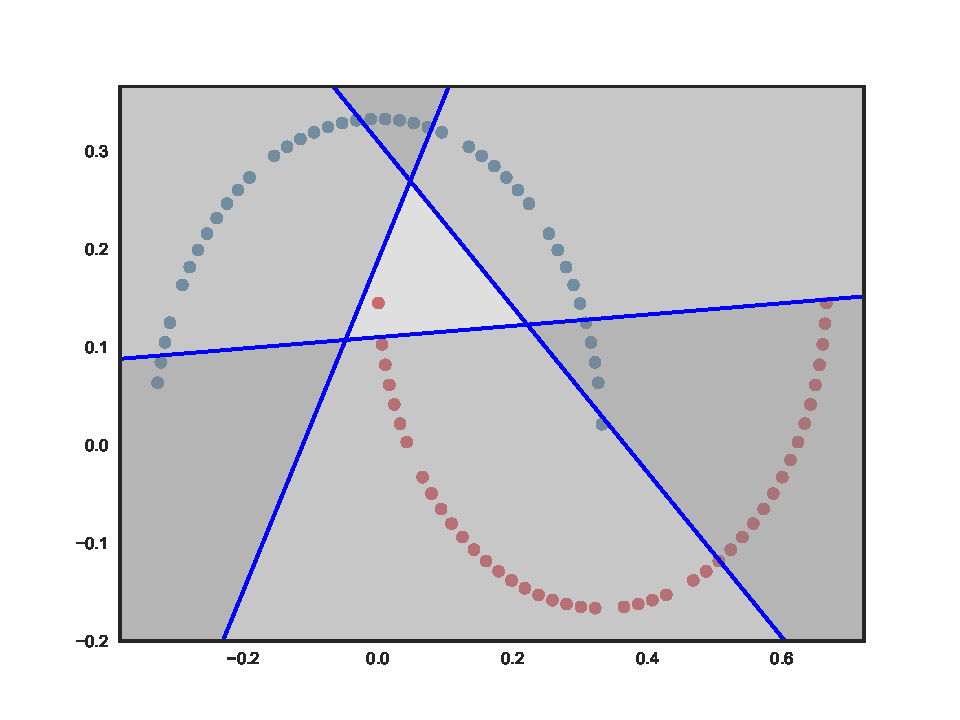
\includegraphics[width=\hsize]{img/toy/layerwise/conv2d_1-0.pdf}}
    }
    % \hskip1em
    \parbox{.195\textwidth}{%
      \subcaptionbox{4th layer\label{fig:moonsLayerwise41}}{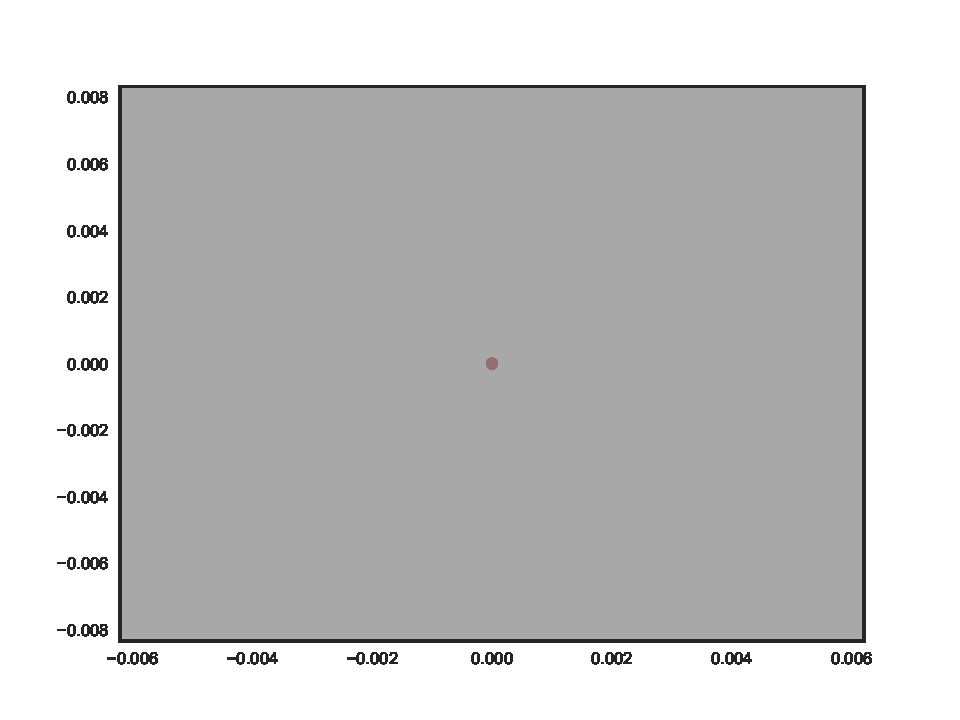
\includegraphics[width=\hsize]{img/toy/layerwise/conv2d_4-0.pdf}}
    %   \vskip1em
      \subcaptionbox{4th layer\label{fig:moonsLayerwise42}}{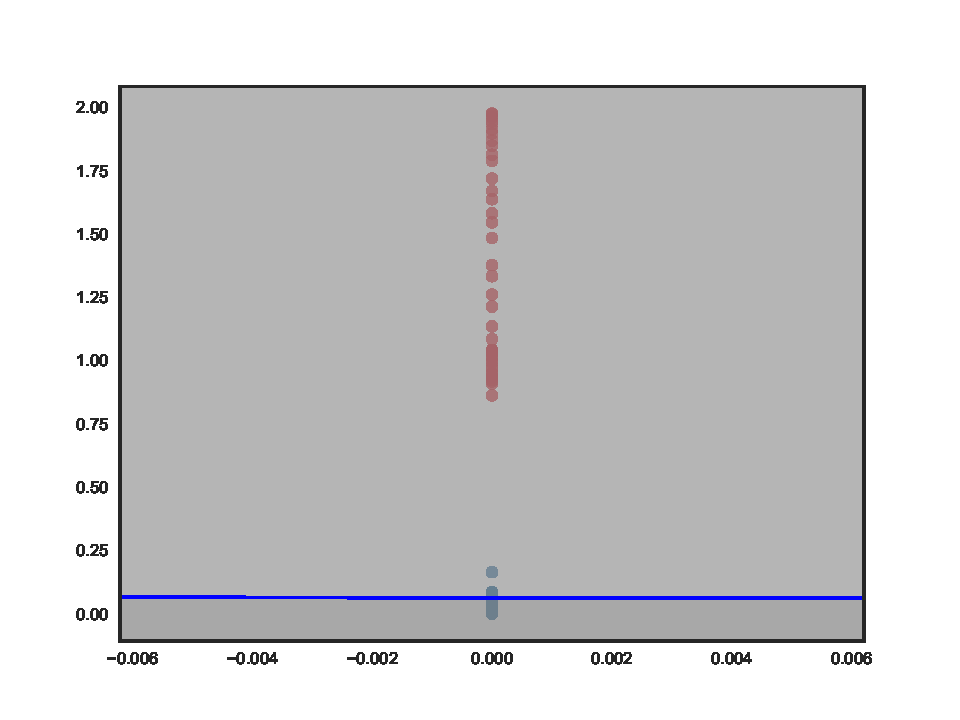
\includegraphics[width=\hsize]{img/toy/layerwise/conv2d_4-2.pdf}} 
    }
    % \hskip1em
    \parbox{.195\textwidth}{%
      \subcaptionbox{25th layer\label{fig:moonsLayerwise251}}{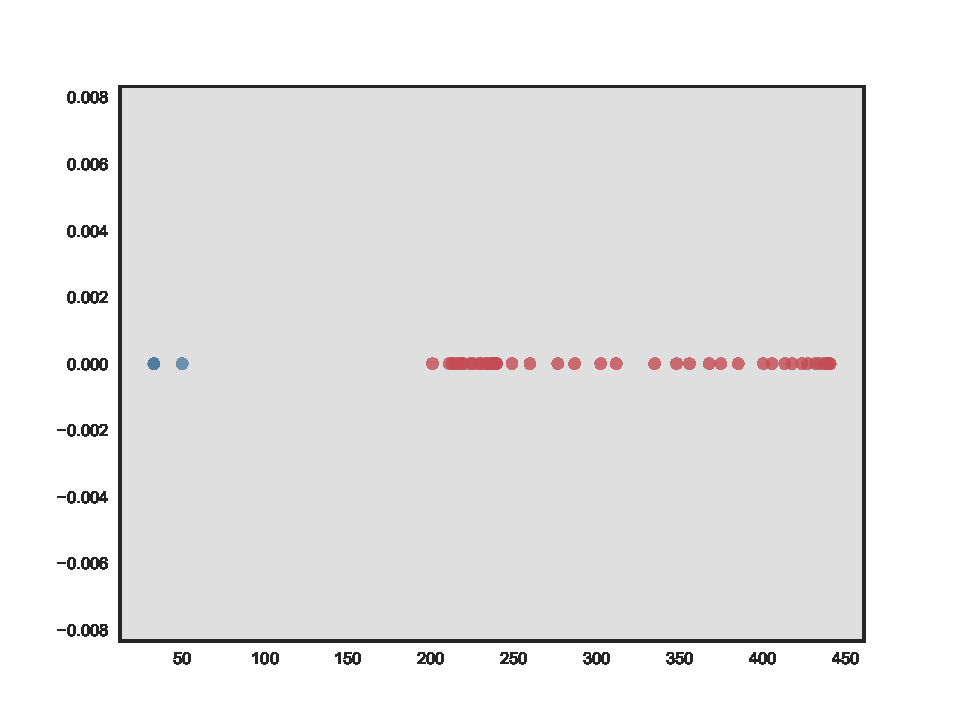
\includegraphics[width=\hsize]{img/toy/layerwise/conv2d_25-0.pdf}}
    %   \vskip1em
      \subcaptionbox{25th layer\label{fig:moonsLayerwise252}}{\includegraphics[width=\hsize]{img/toy/layerwise/conv2d_25-2.pdf}} 
    }
    % \hskip1em
    \parbox{.195\textwidth}{%
      \subcaptionbox{Feature layer\label{fig:moonsLayerwiseFeature1}}{\includegraphics[width=\hsize]{img/toy/layerwise/dense_1-0.pdf}}
    %   \vskip1em
      \subcaptionbox{Feature layer\label{fig:moonsLayerwiseFeature2}}{\includegraphics[width=\hsize]{img/toy/layerwise/dense_1-2.pdf}} 
    }
    % \hskip1em
    \parbox{.195\textwidth}{%
      \subcaptionbox{Output\label{fig:moonsLayerwiseOutput}}{\includegraphics[clip, trim=2.35cm 1.75cm 4.5cm 0cm,width=\hsize]{img/toy/layerwise/output.pdf}}
    }
  }
    \caption{Data transformed across a 50x4 \SepLayer network. Although being a relaxation of \SepUnitPoint showing an intuitive solution with several affine and dead units. Indeed, they not only do not hinder the network but forward the solution 4th layer to the output.}
    \label{fig:moonsLayerwise}
\end{figure*}

\begin{figure*}[h!]
  \centering
    \begin{subfigure}[b]{0.3\textwidth}
        \includegraphics[width=\textwidth]{img/init/relu/conv2d_1-0.pdf}
        \caption{\ReLU input layer}
        \label{fig:reluInitInput}
    \end{subfigure}
    ~ %add desired spacing between images, e. g. ~, \quad, \qquad, \hfill etc. 
      %(or a blank line to force the subfigure onto a new line)
    \begin{subfigure}[b]{0.3\textwidth}
        \includegraphics[width=\textwidth]{img/init/relu/conv2d_50-0.pdf}
        \caption{\ReLU 50th layer}
        \label{fig:reluInit501}
    \end{subfigure}
    ~ %add desired spacing between images, e. g. ~, \quad, \qquad, \hfill etc. 
    %(or a blank line to force the subfigure onto a new line)
    \begin{subfigure}[b]{0.3\textwidth}
        \includegraphics[width=\textwidth]{img/init/relu/conv2d_50-2.pdf}
        \caption{\ReLU 50th layer}
        \label{fig:reluInit502}
    \end{subfigure}
    \\
    \begin{subfigure}[b]{0.3\textwidth}
        \includegraphics[width=\textwidth]{img/init/relu-bn/conv2d_1-0.pdf}
        \caption{\ReLUBN input layer}
        \label{fig:reluBNInitInput}
    \end{subfigure}
    ~ %add desired spacing between images, e. g. ~, \quad, \qquad, \hfill etc. 
      %(or a blank line to force the subfigure onto a new line)
    \begin{subfigure}[b]{0.3\textwidth}
        \includegraphics[width=\textwidth]{img/init/relu-bn/conv2d_50-0.pdf}
        \caption{\ReLUBN 50th layer}
        \label{fig:reluBNInit501}
    \end{subfigure}
    ~ %add desired spacing between images, e. g. ~, \quad, \qquad, \hfill etc. 
    %(or a blank line to force the subfigure onto a new line)
    \begin{subfigure}[b]{0.3\textwidth}
        \includegraphics[width=\textwidth]{img/init/relu-bn/conv2d_50-2.pdf}
        \caption{\ReLUBN 50th layer}
        \label{fig:reluBNInit502}
    \end{subfigure}
    \\
    \begin{subfigure}[b]{0.3\textwidth}
        \includegraphics[width=\textwidth]{img/init/layerwise/conv2d_1-0.pdf}
        \caption{\SepLayer input layer}
        \label{fig:layerwiseInitInput}
    \end{subfigure}
    ~ %add desired spacing between images, e. g. ~, \quad, \qquad, \hfill etc. 
      %(or a blank line to force the subfigure onto a new line)
    \begin{subfigure}[b]{0.3\textwidth}
        \includegraphics[width=\textwidth]{img/init/layerwise/conv2d_50-0.pdf}
        \caption{\SepLayer 50th layer}
        \label{fig:layerwiseInit501}
    \end{subfigure}
    ~ %add desired spacing between images, e. g. ~, \quad, \qquad, \hfill etc. 
    %(or a blank line to force the subfigure onto a new line)
    \begin{subfigure}[b]{0.3\textwidth}
        \includegraphics[width=\textwidth]{img/init/layerwise/conv2d_50-2.pdf}
        \caption{\SepLayer 50th layer}
        \label{fig:layerwiseInit502}
    \end{subfigure}
    \\
    \begin{subfigure}[b]{0.3\textwidth}
        \includegraphics[width=\textwidth]{img/init/unitpointwise/conv2d_1-0.pdf}
        \caption{\SepUnitPoint Input}
        \label{fig:unitpointInitInput}
    \end{subfigure}
    ~ %add desired spacing between images, e. g. ~, \quad, \qquad, \hfill etc. 
      %(or a blank line to force the subfigure onto a new line)
    \begin{subfigure}[b]{0.3\textwidth}
        \includegraphics[width=\textwidth]{img/init/unitpointwise/conv2d_50-0.pdf}
        \caption{\SepUnitPoint 50th layer}
        \label{fig:unitpointInit501}
    \end{subfigure}
    ~ %add desired spacing between images, e. g. ~, \quad, \qquad, \hfill etc. 
    %(or a blank line to force the subfigure onto a new line)
    \begin{subfigure}[b]{0.3\textwidth}
        \includegraphics[width=\textwidth]{img/init/unitpointwise/conv2d_50-2.pdf}
        \caption{\SepUnitPoint 50th layer}
        \label{fig:unitpointInit502}
    \end{subfigure}
    
  \caption{Data transformed across a 50x4 network with no main loss (cross-entropy) with constraints \SepLayer and \SepUnitPoint, versus \ReLU and \ReLUBN. Notice how effectively \ReLU and \ReLUBN collapse the dataset into few points whereas \SepLayer and \SepUnitPoint force the network to learn representations that preserve geometrical structure useful for back-propagation.} 
  \label{fig:init} 
\end{figure*}

\subsection{Dynamic Behavior of the constraints}\label{subsec:dynamicBehavior}
\begin{figure*}[h!]
    \begin{subfigure}[c]{1\textwidth}
        \centering
        \includegraphics[width=1\textwidth]{img/convergence/peaks_loss.pdf}
        \caption{Evolution of cross-entropy and constraint loss during training.}
        \label{fig:loss_convergence}
    \end{subfigure}
    \\
    \begin{subfigure}[c]{1\textwidth}
        \centering
        
            \includegraphics[width=1\textwidth]{img/convergence/peaks_acc.pdf}
        \caption{Evolution of accuracy during training.}
        \label{fig:accuracy_convergence}
    \end{subfigure}
    \\
     
\begin{subfigure}[b]{0.0325\textwidth}
    \begin{tikzpicture}
    \node[remember picture,anchor=south west,inner sep=0] (1154) at (0,0) {\includegraphics[clip, trim=2.35cm 1.75cm 4.5cm 0cm,width=1.1\textwidth]{img/convergence/1154.pdf}};
    \end{tikzpicture}
    \label{fig:convergence_1154}
\end{subfigure}
%
\begin{subfigure}[b]{0.0325\textwidth}
    \includegraphics[clip, trim=2.35cm 1.75cm 4.5cm 0cm,width=1.1\textwidth]{img/convergence/2400.pdf}
    \label{fig:convergence_2400}
\end{subfigure}
%
\begin{subfigure}[b]{0.0325\textwidth}
    \includegraphics[clip, trim=2.35cm 1.75cm 4.5cm 0cm,width=1.1\textwidth]{img/convergence/6200.pdf}
    \label{fig:convergence_6200}
\end{subfigure}
%
\begin{subfigure}[b]{0.0325\textwidth}
    \includegraphics[clip, trim=2.35cm 1.75cm 4.5cm 0cm,width=1.1\textwidth]{img/convergence/6205.pdf}
    \label{fig:convergence_6205}
\end{subfigure}
%
\begin{subfigure}[b]{0.0325\textwidth}
    \includegraphics[clip, trim=2.35cm 1.75cm 4.5cm 0cm,width=1.1\textwidth]{img/convergence/7200.pdf}
    \label{fig:convergence_7200}
\end{subfigure}
%
\begin{subfigure}[b]{0.0325\textwidth}
    \includegraphics[clip, trim=2.35cm 1.75cm 4.5cm 0cm,width=1.1\textwidth]{img/convergence/8123.pdf}
    \label{fig:convergence_8123}
\end{subfigure}
%
\begin{subfigure}[b]{0.0325\textwidth}
    \includegraphics[clip, trim=2.35cm 1.75cm 4.5cm 0cm,width=1.1\textwidth]{img/convergence/8132.pdf}
    \label{fig:convergence_8132}
\end{subfigure}
%
\begin{subfigure}[b]{0.0325\textwidth}
    \includegraphics[clip, trim=2.35cm 1.75cm 4.5cm 0cm,width=1.1\textwidth]{img/convergence/8264.pdf}
    \label{fig:convergence_8264}
\end{subfigure}
%
\begin{subfigure}[b]{0.0325\textwidth}
    \includegraphics[clip, trim=2.35cm 1.75cm 4.5cm 0cm,width=1.1\textwidth]{img/convergence/8344.pdf}
    \label{fig:convergence_8344}
\end{subfigure}
%
\begin{subfigure}[b]{0.0325\textwidth}
    \includegraphics[clip, trim=2.35cm 1.75cm 4.5cm 0cm,width=1.1\textwidth]{img/convergence/9161.pdf}
    \label{fig:convergence_9161}
\end{subfigure}
%
\begin{subfigure}[b]{0.0325\textwidth}
    \includegraphics[clip, trim=2.35cm 1.75cm 4.5cm 0cm,width=1.1\textwidth]{img/convergence/9179.pdf}
    \label{fig:convergence_9179}
\end{subfigure}
%
\begin{subfigure}[b]{0.0325\textwidth}
    \includegraphics[clip, trim=2.35cm 1.75cm 4.5cm 0cm,width=1.1\textwidth]{img/convergence/11883.pdf}
    \label{fig:convergence_11883}
\end{subfigure}
%
\begin{subfigure}[b]{0.0325\textwidth}
    \includegraphics[clip, trim=2.35cm 1.75cm 4.5cm 0cm,width=1.1\textwidth]{img/convergence/11886.pdf}
    \label{fig:convergence_11886}
\end{subfigure}
%
\begin{subfigure}[b]{0.0325\textwidth}
    \includegraphics[clip, trim=2.35cm 1.75cm 4.5cm 0cm,width=1.1\textwidth]{img/convergence/12584.pdf}
    \label{fig:convergence_12584}
\end{subfigure}
%
\begin{subfigure}[b]{0.0325\textwidth}
    \includegraphics[clip, trim=2.35cm 1.75cm 4.5cm 0cm,width=1.1\textwidth]{img/convergence/14000.pdf}
    \label{fig:convergence_14000}
\end{subfigure}
%
\begin{subfigure}[b]{0.0325\textwidth}
    \includegraphics[clip, trim=2.35cm 1.75cm 4.5cm 0cm,width=1.1\textwidth]{img/convergence/14022.pdf}
    \label{fig:convergence_14022}
\end{subfigure}
%
\begin{subfigure}[b]{0.0325\textwidth}
    \includegraphics[clip, trim=2.35cm 1.75cm 4.5cm 0cm,width=1.1\textwidth]{img/convergence/14382.pdf}
    \label{fig:convergence_14382}
\end{subfigure}
%
\begin{subfigure}[b]{0.0325\textwidth}
    \includegraphics[clip, trim=2.35cm 1.75cm 4.5cm 0cm,width=1.1\textwidth]{img/convergence/14457.pdf}
    \label{fig:convergence_14457}
\end{subfigure}
%
\begin{subfigure}[b]{0.0325\textwidth}
    \includegraphics[clip, trim=2.35cm 1.75cm 4.5cm 0cm,width=1.1\textwidth]{img/convergence/14461.pdf}
    \label{fig:convergence_14461}
\end{subfigure}
%
\begin{subfigure}[b]{0.0325\textwidth}
    \includegraphics[clip, trim=2.35cm 1.75cm 4.5cm 0cm,width=1.1\textwidth]{img/convergence/15600.pdf}
    \label{fig:convergence_15600}
\end{subfigure}
%
\begin{subfigure}[b]{0.0325\textwidth}
    \includegraphics[clip, trim=2.35cm 1.75cm 4.5cm 0cm,width=1.1\textwidth]{img/convergence/16424.pdf}
    \label{fig:convergence_16424}
\end{subfigure}
%
\begin{subfigure}[b]{0.0325\textwidth}
    \includegraphics[clip, trim=2.35cm 1.75cm 4.5cm 0cm,width=1.1\textwidth]{img/convergence/16432.pdf}
    \label{fig:convergence_16432}
\end{subfigure}
%
\begin{subfigure}[b]{0.0325\textwidth}
    \includegraphics[clip, trim=2.35cm 1.75cm 4.5cm 0cm,width=1.1\textwidth]{img/convergence/16435.pdf}
    \label{fig:convergence_16435}
\end{subfigure}
%
\begin{subfigure}[b]{0.0325\textwidth}
    \includegraphics[clip, trim=2.35cm 1.75cm 4.5cm 0cm,width=1.1\textwidth]{img/convergence/16442.pdf}
    \label{fig:convergence_16442}
\end{subfigure}
%
\begin{subfigure}[b]{0.0325\textwidth}
    \includegraphics[clip, trim=2.35cm 1.75cm 4.5cm 0cm,width=1.1\textwidth]{img/convergence/16444.pdf}
    \label{fig:convergence_16444}
\end{subfigure}
%
\begin{subfigure}[b]{0.0325\textwidth}
    \includegraphics[clip, trim=2.35cm 1.75cm 4.5cm 0cm,width=1.1\textwidth]{img/convergence/16630.pdf}
    \label{fig:convergence_16630}
\end{subfigure}
%
\begin{subfigure}[b]{0.0325\textwidth}
    \includegraphics[clip, trim=2.35cm 1.75cm 4.5cm 0cm,width=1.1\textwidth]{img/convergence/16632.pdf}
    \label{fig:convergence_16632}
\end{subfigure}
%
      \caption{Evolution of training throughout epochs (cross-entropy, constraint loss, and accuracy). Left-hand axis show the accuracy metric (blue line) against the cross-entropy, and constraint loss in the right axis (orange line), for each epoch of the training phase in the horizontal axis.}
	\label{fig:peaks}
\end{figure*}
\begin{figure*}[h!]
  \centering
  \begin{subfigure}[b]{0.2\textwidth}
        \includegraphics[width=\textwidth]{img/moons_grid/acc-sep-up-0-0001.pdf}
        \caption{Glorot initialization}
        \label{fig:moons_glorot_rho}
    \end{subfigure}
    ~ %add desired spacing between images, e. g. ~, \quad, \qquad, \hfill etc. 
      %(or a blank line to force the subfigure onto a new line)
      \centering
    \begin{subfigure}[b]{0.2\textwidth}
        \includegraphics[width=\textwidth]{img/moons_grid/acc-sep-up-0-0001-zero.pdf}
        \caption{Zero initialization with $\rho = 0.51$}
        \label{fig:moons_zeros_rho}
    \end{subfigure}
    ~ %add desired spacing between images, e. g. ~, \quad, \qquad, \hfill etc. 
      %(or a blank line to force the subfigure onto a new line)
    \centering
    \begin{subfigure}[b]{0.2\textwidth}
        \includegraphics[width=\textwidth]{img/moons_grid/acc-sep-up-0-0001-nm-0.pdf}
        \caption{Glorot initialization with negative margin to zero}
        \label{fig:moons_glorot_nm0}
    \end{subfigure}
    ~ %add desired spacing between images, e. g. ~, \quad, \qquad, \hfill etc. 
      %(or a blank line to force the subfigure onto a new line)
    \centering
    \begin{subfigure}[b]{0.2\textwidth}
        \includegraphics[width=\textwidth]{img/moons_grid/acc-sep-up-0-0001-nm-0.pdf}
        \caption{Zero initialization with negative margin to zero}
        \label{fig:moons_zeros_nm0}
    \end{subfigure}
    
  \caption{Glorot vs Zero initialization in a series of Depth $D$ vs Width $W$ accuracy plots a for rectangular network using a grid ($2\leq W\leq 25$ and $2\leq D\leq 150$), trained over the \texttt{MOONS} dataset using an Adam learning rate of $0.01$, annealed dropout for $1000$ epoch with an initial rate of $0.01$ in the. The color scheme depicts accuracy attained for each grid location, from dark to light. (a) classical Glorot, (b) Zero intialization using $\rho=0.51$, (c) Glorot initialization using $\rho=0$ or enforcing only non-negative constraints and (d) Zero initialization using $\rho=0$ or non-negative constraints. 
  }
  \label{fig:moons_grid_zero} 
\end{figure*}
     